\documentclass[a4paper,12pt]{extarticle}
\usepackage{geometry}
\usepackage[T1]{fontenc}
\usepackage[utf8]{inputenc}
\usepackage[english,russian]{babel}
\usepackage{amsmath}
\usepackage{amsthm}
\usepackage{amssymb}
\usepackage{fancyhdr}
\usepackage{setspace}
\usepackage{graphicx}
\usepackage{colortbl}
\usepackage{tikz}
\usepackage{pgf}
\usepackage{subcaption}
\usepackage{listings}
\usepackage{indentfirst}
\usepackage[colorlinks,citecolor=blue,linkcolor=blue,bookmarks=false,hypertexnames=true, urlcolor=blue]{hyperref} 
\usepackage[noabbrev]{cleveref}
\usepackage{indentfirst}
\usepackage{mathtools}
\usepackage{booktabs}
\usepackage[flushleft]{threeparttable}
\usepackage{tablefootnote}
% \usepackage{refcheck}

\usepackage{chngcntr} % нумерация графиков и таблиц по секциям
\counterwithin{table}{section}
\counterwithin{figure}{section}
\DeclareMathOperator*{\argmin}{arg\,min} 
\graphicspath{{graphics/}}%путь к рисункам

\makeatletter
\renewcommand{\@biblabel}[1]{#1.} % Заменяем библиографию с квадратных скобок на точку:
\makeatother

\geometry{left=2.5cm}% левое поле
\geometry{right=1.5cm}% правое поле
\geometry{top=1.5cm}% верхнее поле
\geometry{bottom=1.5cm}% нижнее поле
\renewcommand{\baselinestretch}{1.25} % междустрочный интервал
\RequirePackage{float}                

\newcommand{\goal}[0]{\texttt{Goal}}
\newcommand{\prune}[0]{\texttt{Prune}}
\newcommand{\invariant}[0]{\texttt{Invariant}}
\newcommand{\collect}[0]{\texttt{Collect}}
\newcommand{\mc}[0]{MC}

\addto\captionsrussian{\def\refname{Список литературы}} 

\renewcommand{\theenumi}{\arabic{enumi}.}% Меняем везде перечисления на цифра.цифра
\renewcommand{\labelenumi}{\arabic{enumi}.}% Меняем везде перечисления на цифра.цифра
\renewcommand{\theenumii}{\arabic{enumii}.}% Меняем везде перечисления на цифра.цифра
\renewcommand{\labelenumii}{\arabic{enumi}.\arabic{enumii}.}% Меняем везде перечисления на цифра.цифра
\renewcommand{\theenumiii}{\arabic{enumiii}.}% Меняем везде перечисления на цифра.цифра
\renewcommand{\labelenumiii}{\arabic{enumi}.\arabic{enumii}.\arabic{enumiii}.}% Меняем везде перечисления на цифра.цифра

\crefname{section}{глава}{глава }
\Crefname{section}{Глава}{Глава }
\crefname{figure}{рис.}{рис. }
\Crefname{figure}{Рис.}{Рис. }
\crefname{table}{табл.}{табл. }
\Crefname{table}{Табл.}{Табл. }

\begin{document}
\begin{titlepage}
    \newpage
    
    {\setstretch{1.0}
    \begin{center}
    Федеральное государственное автономное образовательное \\
    учреждение высшего образования \\
    \vspace{1em}
    <<Национальный исследовательский университет \\
    <<Высшая школа экономики>>
    \\
    \vspace{4em}
    Факультет компьютерных наук \\
    \vspace{1em}
    Основная образовательная программа \\
    Прикладная математика и информатика \\
    \end{center}
    }
    
    \vspace{10em}
    
    \begin{center}
        \textbf{ВЫПУСКНАЯ КВАЛИФИКАЦИОННАЯ РАБОТА}
        \vspace{2em}
        \\
        \textbf{
            Программный проект на тему
            \linebreak
            <<Использование model checking для тестирования распределенных систем в фреймворке DSLab>>
        }
    \end{center}
    
    \vspace{8em}
    
    {\setstretch{1.0}
    \hfill\parbox{16cm}{
    \hspace*{5cm}\hspace*{-5cm}Выполнил студент группы БПМИ 195, 4 курса,\\
    Амеличев Константин Вадимович\\
     
    \hspace*{5cm}\hspace*{-5cm}Руководитель ВКР:\\
    Доцент, к.т.н., ФКН ВШЭ, Сухорослов Олег Викторович\\
    
    %\hspace*{5cm}\hspace*{-5cm}Куратор:\hfill < степень>, <звание>, <ФИО полностью>\\
    }
    }
    
    \vspace{\fill}

\begin{center}
Москва 2023
\end{center}
    
\end{titlepage}% это титульный лист
\newpage

{
	\hypersetup{linkcolor=black}
	\tableofcontents
}

\newpage

\textbf{Аннотация}

При тестировании распределенных систем возникает необходимость проверить все возможные ситуации, в которых может оказаться система.
Данная работа ставит целью использовать model checking, один из формальных методов для тестирования распределенных систем, в рамках лабораторных и домашних заданий курса <<Распределенные системы>>, реализованных в симуляционном фреймворке DSLab.
Работа предлагает оптимизации для метода model checking, модуль DependencyResolver, а также несколько специальных режимов: Instant и Collect Mode.
С помощью предложенных методов было найдено более 10 новых ошибок в архивных решениях заданий.

\textbf{Ключевые слова:} Model checking, распределенные системы, автоматическое тестирование,  дискретно-событийное моделирование.

\hfill

\textbf{Annotation}

During the testing of distributed systems, it is crucial to examine all possible states that the system can get into.
This research uses model checking as a formal method to test distributed systems within the context of the <<Distributed Systems>> course assignments.
The simulations are conducted using the DSLab framework.
We propose various optimizations for model checking, including the DependencyResolver module, as well as the introduction of two special workflows: Instant and Collect modes.
These methods have successfully discovered over 10 previously unknown bugs in the archive of assignment solutions.

\textbf{Keywords:} Model checking, distributed systems, automated software testing, discrete event simulation.

\newpage

\section{Введение}

Современным компьютерным системам требуется обрабатывать запросы большого количества пользователей и работать под высокой нагрузкой.
Появляется необходимость в распределенных системах, которые за счет кооперативной работы могут обойти ограничения в ресурсах, существующие для одного сервера.
В то же время распределенные системы сложнее поддерживать и разрабатывать, особенно когда они начинают состоять из сотен или тысяч узлов.

В распределенных системах основным источником ошибок являются аппаратные и сетевые сбои, за счет которых нарушается синхронизация и обмен сообщениями между узлами в системе.
Для того чтобы неожиданный сбой не нарушил работу сервиса, необходимо полное тестирование корректности распределенной системы.

Данная работа исследует методы формальной верификации для распределенных систем.
Основным методом формальной верификации распределенной системы в данной работе является метод model checking (сокращенно \mc).
Работа выполнена на основе фреймворка DSLab \cite{b12} и его модуля DSLab-MP, который применяется для симуляции распределенных систем.
DSLab является потомком фреймворка dslib \cite{b11}, который используется для тестирования заданий курса "Распределенные системы" в Высшей школе экономики.

\subsection{Актуальность и значимость работы}


Каждое задание в рамках курса <<Распределенные системы>> требует от студента реализовать логику для процессов, соответствующую требованиям задачи.
В задаче есть набор тестов, каждый из которых отправляет набор запросов и ожидает от системы корректные ответы на запросы.
Некоторые тесты сделаны так, чтобы в промежуточный момент узел вышел из строя или сеть потеряла сообщение.
Такое искусственное внедрение отказов помогает найти ошибки в коде студента.
Также существуют рандомизированные тесты, которые выполняются много раз с разным случайным параметром, чтобы более тщательно проверить систему.
Такие тесты в рамках заданий называются <<chaos monkey>> тестами.

Описанные выше тесты, к сожалению, не могут проверить, что решение студента корректно работает при любом возможном выполнении.
Для того чтобы формально проверить прохождение даже базового теста, нужно использовать формальные методы, такие как \mc.
Более тщательная проверка студенческих решений приведет к улучшению навыков разработки и отладки распределенных систем у студентов, выполнявших задание.

\subsection{Цели и задачи ВКР}

Целью ВКР было улучшение тестов к практическим заданиям в фреймворке DSLab на основе метода model checking.

Для достижения этой цели были поставлены следующие задачи:

\begin{enumerate}
    \item Изучение метода \mc\ и его применения для тестирования распределенных систем
    \item Доработка ядра \mc\ в DSLab
    \item Перенос заданий курса <<Распределенные системы>> на базу фреймворка DSLab
	\item Разработка тестов к домашним заданиям по курсу <<Распределенные системы>> с использованием \mc
	\item Анализ производительности тестов на основе \mc
    \item Тестирование архивных студенческих решений на тестах в режиме \mc\ и анализ найденных ошибок в решениях
\end{enumerate}


\subsection{Основные результаты работы}

Данная работа развивает применение \mc\ в образовательных проектах, приводит опыт использования \mc\ в новых типах заданий, а также предлагает дополнительные режимы для тестирования распределенных систем.
Благодаря тестам к практическим заданиям было обнаружено больше 10 различных типов ошибок, которые не были найдены оригинальными тестами.

\subsection{Структура работы}

Дальнейшая структура работы выглядит следующим образом:

\begin{itemize}
\item \Cref{CHAPTER2} вводит модель распределенной системы, которая используется в работе, приводит обзор методов формальной верификации распределенной системы, а также приводит опыт использования таких методов в образовательных проектах.
\item \Cref{CHAPTER3} описывает реализацию model checking в DSLab, его функционал, ядро и модули.
\item \Cref{CHAPTER4} описывает подготовленные тесты к домашним заданиям в режиме model checking, найденные с помощью \mc\ ошибки в студенческих решениях, а также содержит общие рекомендации по написанию тестов к заданиям в режиме \mc.
\item \Cref{CHAPTER5} подводит итоги работы и предлагает дальнейшие направления работы над \mc\ в DSLab. 
\end{itemize}

\section{Обзор литературы}
\label{CHAPTER2}

Существует большое количество способов протестировать корректность программы: ручные и автоматические тесты в разных окружениях, с искусственным внедрением ошибок и случайными конфигурациями.
Но такие методы не могут гарантировать корректность распределенной системы, они могут только увеличить уверенность, что она работает так, как от нее ожидается.
Существуют более надежные методы проверки корректности системы, которые будут рассмотрены в данной главе.

Также в главе описана использующаяся модель распределенной системы и приведен обзор образовательных проектов, использующих \mc.

\subsection{Модель распределенной системы в DSLab-MP}

Распределенная система состоит из набора узлов, каждый из которых соответствует серверу с запущенным инстансом сервиса.
DSLab-MP дает возможность симуляции отказа узлов и потери сообщений в сети.

На каждом узле запущен набор процессов.
Процессы могут отправлять сообщения друг другу.
Если сообщение отправлено процессу на другом узле, сообщение пройдет через модель сеть, которая эмулирует реальное сетевое соединение.
Сеть может эмулировать отказы, задержку или дубликацию сообщений.
Также процессы могут использовать таймеры для отложенных действий и отправлять сообщения в локальный лог.

Реализация каждого процесса выполняется в actor-based модели \cite{b21}.
Конфигурация актора предполагает определение набора методов, каждый из которых будет вызываться в определенных случаях.
Актор процесса реализует несколько методов:

\begin{enumerate}
\item \texttt{on\_local\_message}, реагирующий на получение сообщения от клиента системы. Он отвечает за обработку запросов.
\item \texttt{on\_message}, реагирующий на получение сообщения по сети.
\item \texttt{on\_timer}, реагирующий на срабатывание таймера.
\end{enumerate}

DSLab использует дискретно-событийное моделирование, чтобы моделировать работу распределенной системы.
В симуляции существует несколько типов событий.
Два основных типа события~--- срабатывание таймера и доставка сообщения по сети.
Такие события хранятся в очереди с приоритетами и симуляция шаг за шагом продвигается по времени путем обработки события с минимальным значением времени.

В дальнейшей работе термин \textit{состояние распределенной системы} используется, чтобы описать множество, содержащее в себе состояние всех процессов, состояние сети, события в симуляции.
Термином \textit{траектория исполнения} будет обозначаться последовательность состояний, связанных между собой последовательным прибавлением событий.
Можно считать, что каждая траектория исполнения является возможной последовательностью событий в системе, приводящую систему в заданное состояние.

\subsection{Формальная спецификация распределенной системы}

Корректность распределенной систему можно показать, записав ее на формальном языке, позволяющем явно сконструировать доказательство.
Примером такого языка для формальной спецификации является $\text{TLA}^+$, который активно используется в Amazon \cite{b31, b4}.

\subsubsection{$\text{TLA}^+$}

$\text{TLA}^+$ предлагает набор предикатов, которым можно описать свойства системы, и набор правил, которым можно разложить спецификацию из одной формулы с сотней параметров в набор модулей и предикатов.
В экосистеме $\text{TLA}^+$ предлагается программное обеспечение, проверяющее корректность спецификации \cite{b33}.

Такой подход, к сожалению, не подойдет для проверки заданий в рамках курса <<Распределенные системы>> по нескольким причинам.
Спецификация и реализация в большинстве случаев пишутся на разных языках, а значит, между ними создается разрыв, который может влиять на корректность.
Кроме этого, написание спецификации на формальном языке является сложной задачей, которая выходит за рамки умений студентов третьего курса.

\subsubsection{Verdi}

Существует фреймворк Verdi \cite{b3}, решающий одну из проблем $\text{TLA}^+$~--- существование разницы между спецификацией и реализацией.
Verdi построен поверх языка Coq \cite{b35}, который позволяет строить одновременно формальное доказательство и исполняемый файл.
Поскольку язык Coq ориентирован на формальные доказательства, реализации распределенных систем на Verdi (например, алгоритма Raft \cite{b34}) достаточно специфичны и сильно отличаются от промышленных реализаций.
За счет этого разработка на Verdi отличается от разработки распределенных систем, которые можно было бы использовать в практических целях.

Таким образом, было решено отказаться от формальной спецификации в пользу методов, которые пользуются только исходным кодом приложения.

\subsection{Model checking}

Model checking является методом проверки всех возможных путей исполнения теста в рамках системы.
Он используется для тестирования многопоточных приложений и распределенных систем \cite{b23,b22}.

\mc\ не дает формального доказательства, что система корректна, потому что делает исчерпывающее тестирование только для одного конкретного теста.
Тем не менее исследования \cite{b9} показывают, что большинство ошибок в распределенных системах можно отловить в сравнительно небольших окружениях.
Таким образом, прохождение даже небольшого теста в режиме  \mc\ является весомым аргументом в пользу того, что система корректна.

Ниже приводится обзор промышленных model checker-ов для распределенных систем и многопоточных приложений, а также методов и техник, которые используют данные системы.

\subsubsection{CBSChecker}

CBSChecker --- это система, реализующая \mc\ для программ на языке C++ \cite{b5}.
Данная система проверяет работоспособность многопоточных приложений в модели памяти C++.
Для этого авторы анализируют поведение атомиков в C++, вводят отношения событий, примерами которых являются sequenced-before и happenes-before.
В построенной модели памяти можно выделить набор ограничений, которые авторы используют для ускорения обхода графа состояний.
Благодаря CBSChecker удалось найти ряд ошибок в ряде примитивов для многопоточной работы.

Похожие рассуждения о зависимости событий используются в главе \ref{dependencies}.
Благодаря анализу отношения happenes-before для модели распределенной системы получилось добавить набор оптимизаций в DSLab, а также убрать определенные невалидные состояния из траекторий \mc. 


\subsubsection{FlyMc}

Проект FlyMc \cite{b6} является одним из самых эффективных на текущий момент model checker-ов для распределенных систем.

FlyMc предлагает три оптимизации для техники \mc, которые в комбинации дают достаточно высокий прирост в производительности, чтобы находить десятки ошибок в таких популярных системах, как Zookeeper \cite{b7} и Spark \cite{b8}.

Первой техникой является обработка симметричных состояний.
Состояния считаются симметричными, если их история различна, но сами по себе состояния не отличаются от уже рассмотренных.
Такое может быть возможно, например, при перенумеровании процессов.
Также возможны ситуации, когда в силу особенностей системы состояния, которые были получены разными тракеториями, обладают одинаковыми свойствами.

Второй техникой является отслеживание независимых событий.
Такие события могут обрабатываться системой в любом порядке, за счет чего можно фиксировать перестановки таких событий и кратно уменьшать размер графа состояний.
Примером независимых событий в системе может быть доставка сообщений между двумя парами узлов. 

Третьей техникой являются параллельные свапы событий в траектории исполнения.
Эта оптимизация помогает перебирать траектории в произвольном порядке и раньше находить ошибки в системе.

Данная работа пользуется аналогичными техниками сжатия эквивалентных состояний (\cref{visitedstates}), а также частных случаев симметричных состояний (\cref{BROADCAST}) и применения независимых событий (\cref{equalmessages}).



\subsubsection{MaceMC}

\mc\ применяется в основном для проверки safety-свойств системы, то есть для таких свойств, которые могут быть нарушены в конкретном состоянии системы \cite{b30}.
Проверка liveness-свойств является более сложной задачей, потому что \mc\ в первую очередь проверяет свойства конкретного состояния, а свойство liveness относится к траекториям исполнения.
Тем не менее существуют адаптации \mc\ для проверки liveness, такие, как MaceMC \cite{b19}.

MaceMC использует комбинацию ограниченного по глубине DFS и случайного обхода для проверки достижения корректного состояния в конечном счете.
\mc\ сначала обходит все состояния на ограниченной глубине.
Траектории, в которых liveness-свойство еще не стабилизировалось, выбираются в качестве интересных для дальнейшего изучения.
Среди них берется случайная выборка, и из них запускается случайный обход, который в каждом состоянии переходит по случайному событию.
Если все обходы закончились выполнением liveness-свойства, то считается, что это свойство выполнено.

Если обход нашел траекторию, у которой liveness-свойство не выполнилось, происходит изучение траектории.
С помощью траекторий с общим началом находится промежуток событий, в котором система, вероятно, нарушило свои инварианты и тем самым потеряло свое liveness-свойство.

В данной работе была проведена подготовительная работа для подготовки тестов в режиме Random Walk (\cref{MEMBERSHIP}).

Также заметим, что авторы выделяют в своей работе идею, что liveness-свойство часто можно преобразовать в набор safety-свойств.
Такие safety-свойства, к сожалению, сложно задать, имея только определение liveness-свойства.
Зато при нарушении liveness-свойства часто можно выделить нарушенное safety-свойство и в будущем проверять именно его.
Аналогичный вывод был сформулирован в данной работе после создания тестов в режиме \mc касательно ошибок в системе, которые этими тестами находятся (\cref{posteriori}).




\subsection{Model checking в образовательных проектах}

В курсах по распределенным системам возникает необходимость тестирования студенческих решений.
Выделим особенности тестирования практических заданий, а не промышленных систем:
\begin{enumerate}
\item Практические задания по распределенным системам в большинстве случаев предлагают заготовку решения и формат взаимодействия пользователя (или тестирующей программы) с системой.
Заготовка решения для возможности тщательного тестирования, реализуется в рамках некоторого фреймворка.
За счет этого при тестировании учебных заданий у фреймворка без дополнительных модификаций есть необходимый контроль над поведением распределенной системы, позволяющий тестировать работу системы при различных видах отказов.
\item У промышленной системы одна реализация (помимо, возможно, имитирующих ее заглушек).
Реализация одной и той же системы у каждого студента своя.
Это значит, что тестирование системы должно проводиться без опоры на знание исходного кода процессов или нижележащего алгоритма, рассматривая исключительно внешнее поведение системы.  
\end{enumerate}

\subsubsection{DSLabs}

Существует образовательный фреймворк DSLabs \cite{b1} для симуляции распределенных систем.
DSLabs, в отличие от DSLab, уже использует \mc\ для тестирования лабораторных работ (\cref{dslabsmc}).
Помимо стандартного обхода графа исполнения, авторы используют технику punctuate search, чтобы запускать \mc\ из промежуточного состояния системы, из которого нахождение ошибок более вероятно.
% Также авторы утверждают, что в ситуациях, когда граф исполнений бесконечен, глубина исследования графа должна соответствовать глубине, на которой лежат финальные состояния.
% Ведь если система некорректно себя ведет при другом порядке исполнения действий, соответствующее некорректное состояние окажется на сравнимой глубине.

Можно видеть, что лабораторные 3 и 4 (являющиеся самими объемными заданиями) не протестированы в полном объеме.
Это связано с большим размером графа исполнения.
Для увеличения уверенности в корректности системы используется punctuated search и длительное выполнение с отсечением по времени. 

Данная работа во многом опирается на опыт DSLabs, реализуя подавляющее большинство функционала \mc\ в DSLabs.
Также развиваются некоторые идеи и появляется дополнительный функционал.
Например, punctuated search, который предлагает авторы, заменяется режимом \collect (\cref{collect}), который предлагает более исчерпывающий обход графа.
А очередь таймеров, которую авторы используют для отслеживания доступных событий, заменяется на \texttt{DependencyResolver}, который предлагает большее количество оптимизаций и режимов (\ref{dependencies}).

\begin{table}[htbp]
    \caption{Лабораторные в DSLabs}
    \begin{center}
    \begin{tabular}{|c|c|c|}
    \hline
    \textbf{Название} & \textbf{Статус model checking} & \textbf{Размер решения, LOC}  \\
    \hline
    0-pingpong &  полный & 10 \\
    \hline
    1-clientserver & полный & 75 \\
    \hline
    2-primarybackup & полный &  300 \\
    \hline
    3-paxos  & неполный & 400 \\
    \hline
    4-shardedstore & неполный & 1050 \\
    \hline

    \end{tabular}
    \label{dslabsmc}
    \end{center}
\end{table}

\subsubsection{Columbia University}

В курсе Distributed Systems Fundamentals, проводящемся в Columbia University, одним из домашних заданий является создание тестов для алгоритма Paxos с использованием метода \mc\ \cite{b20}.
Данное задание предполагает изучение студентами \mc\ и адаптацию собственной реализации Paxos в формате актора.
Благодаря этому заданию студенты формализуют ранее написанный алгоритм Paxos и тестируют его с помощью \mc.

Нужно заметить что такое применение \mc\ завязано на конкретное задание и не является методом, который можно будет применить в тестировании других домашних заданий.

\subsubsection{dslib}

Данной работе предшествовали работы по внедрению \mc\ для тестирования заданий курса <<Распределенные системы>> в фреймворк dslib \cite{b10,b32}.

Обе предшествующие работы фокусируются на разработке модуля, отвечающего за тестирование в режиме \mc, в рамках фреймворка dslib.
Итогами этих работ можно считать основное ядро компоненты \mc, которое было позже перенесено в DSLab.
Предыдущий опыт использования \mc\ в тестах в первую очередь проверял корректность реализации \mc\ и возможностей техники.

Текущая работа продолжает работу предшественников, но фокусируется не на технике \mc\ как таковой, а на модификациях \mc\ для тестирования практических заданий и подготовке тестов к заданиям.


\subsection{Выводы}

Для тестирования распределенных систем и получения формального подтверждения корректности решения можно использовать различные методы.
Был выбран метод \mc, так как подготовка решения к тестированию в режиме \mc\ не потребует дополнительной разработки от студента.
Помимо этого, интерпретация результата \mc\ прозрачна для студента --- при выявлении ошибочного поведения \mc\ позволяет в явном виде показать последовательность событий, которая привела к ошибке.

Были изучены различные промышленные программы для формальной верификации программ с целью поиска оптимизаций, которые можно использовать при работе над тестами к практическим заданиям.

Существуют случаи успешного использования \mc\ в образовательных проектах, но соответствующие реализации \mc\ оказываются ограничены в возможностях, за счет чего полное тестирование системы невозможно и используется отсечение по времени.
Данная работа предлагает развитие текущих идей, использующихся в образовательных проектах, а также предлагает опыт тестирования архивных студенческих решений. 



\section{Реализация model checking в DSLab-MP}
\label{CHAPTER3}

Режим \mc\ в DSLab получает на вход экземпляр распределенной системы в требуемом для теста начальном состоянии, а потом совершает запуск исчерпывающего поиска.
Ядро \mc\ было реализовано ранее в рамках dslib \cite{b10}, и параллельно с выполнением данной работы шел перенос ядра в DSLab.
При разработке тестов появилась потребность в дополнительных модулях и режимах, которые были добавлены в ядро \mc.


\subsection{McSystem}

Работа с распределенной системой в режиме \mc\ происходит через структуру \texttt{McSystem}.
Система содержит информацию об узлах и процессах, сети, а также информацию о доступных событиях, которые могут произойти в текущий момент времени.
Состоянием системы называется множество состояний процессов и доступных событий.
Система может выдать свое текущее состояние или переключиться на заданное состояние с помощью методов \texttt{get\_state} и \texttt{set\_state}.

Ядро \mc\ позволяет применить к системе любое событие из доступных.
Поскольку \mc\ подразумевает перебор всех возможных траекторий исполнения программы, то перед применением события состояние системы запоминается для будущего использования.
За счет такого подхода в графе исполнений можно делать как переходы <<вперед>> --- с помощью применения события, так и <<назад>> --- с помощью загрузки системы в сохраненное ранее состояние.

\subsection{Сериализация процессов}

Для того чтобы сохранить состояние процесса, нужно понять, какие данные в решении являются важной частью состояния, а какие промежуточной информацией.
Самый первый вариант для сохранения состояния --- это явная реализация методов \texttt{get\_state} и \texttt{set\_state} для процесса.
Но такой подход требует от студента дополнительной сериализации, и этого хочется избежать.
Поскольку базовым языком для написания решений является Python, то сериализация состояния должна в первую очередь работать для него.

Так как любой актор является потомком базового класса \texttt{Process}, было принято решение сделать реализации \texttt{set\_state} и \texttt{get\_state} по умолчанию.
Эти методы считают, что все поля процесса важны для сериализации.
Изучение решений показывает, что это так, потому что данные, не относящиеся к состоянию процесса, обычно помечаются либо как глобальные константы, либо как локальные переменные.

Для реализации \texttt{get\_state} и \texttt{set\_state} используется библиотека pickle \cite{b24}.
С ее помощью любое состояние процесса превращается в строку из латинских символов и цифр с возможностью обратного преобразования (десериализации).

Использование pickle накладывает некоторые ограничения на решения.
Так как pickle сериализует данные по значениям, то согласованность ссылок может оказаться нарушена при десериализации.
Также pickle не сериализует объекты, являющиеся функциями.

Тем не менее эти случаи достаточно редки в студенческих решениях, и их исправление не является сложной задачей для студента, поэтому подобные ограничения вполне допустимы.

\subsection{Стратегии}

\mc\ работает на основе стратегий, определяющих алгоритм обхода графа состояний системы.
Интерфейс стратегии, помимо вспомогательных методов, реализует основной метод \texttt{search\_step}, который получает текущее состояние системы, и пытается создать новые состояния системы путем применения всех возможных событий.
Ядро \mc\ отвечает за то, чтобы применить новое событие, и вызвать \texttt{search\_step} для всех новых состояний системы.

На данный момент реализованы стратегии на основе DFS и BFS, и идет исследование стратегии Random Walk.

При вызове \texttt{search\_step} стратегия DFS по очереди применит каждое из доступных в этом состоянии событий к системе.
Для каждого применения события ядро \mc\ обновит состояние систему и сделает рекурсивный вызов \texttt{search\_step} для нового состояния системы.
При возврате из рекурсии состояние системы вернется в сохраненное на прошлом шаге. 
Таким образом, стратегия DFS задает порядок обхода графа, соответствующий обходу в глубину.

Стратегия BFS обрабатывает события в порядке очереди.
Обработка происходит в одном цикле при вызове метода \texttt{run}, который является основным методом стратегии.
Для каждого состояния в очереди применяется каждое из доступных событий.
При вызове \texttt{search\_step} стратегия BFS добавляет состояние системы в очередь обработки.
Таким образом, стратегия BFS задает порядок обхода графа, соответствующий обходу в ширину.

Также была проведена первичная подготовка стратегии Random Walk.
Стратегия Random Walk при вызове \texttt{search\_step} применяет к системе случайное событие из доступных и делает рекурсивный переход в следующее состояние.
В отличие от стратегий DFS и BFS данная стратегия предлагает вероятностный обход траекторий исполнения, которые могут быть слишком длинными для стратегий с полным обходом графа состояний.
Такой подход может протестировать $n$ случайных траекторий исполнения на корректность.
Это может быть полезно в chaos monkey тестах, которые проверяют решение многократным запуском решения в случайных конфигурациях системы.
Добавление Random Walk позволит тестировать несколько случайных траекторий исполнения для случайных конфигураций систем.  
Дополнительно отметим, что комбинация стратегий DFS и Random Walk может использоваться для тестирования liveness-свойств системы, как это сделано в MACEMC \cite{b19}.



\subsection{Goal, Prune, Invariant}

Для того чтобы кастомизировать стратегии под различные тесты, было принято решение добавить в стратегию методы \goal, \prune, \invariant\ аналогично тому, как это сделано в DSLabs \cite{b1}.
Каждый из этих методов является предикатом, который принимает состояние системы. На основе значений предикатов ядро \mc\ определяет дальнейшую работу алгоритма с состоянием (\cref{mcdiagram}).


\begin{figure}[H]
    \begin{center}
        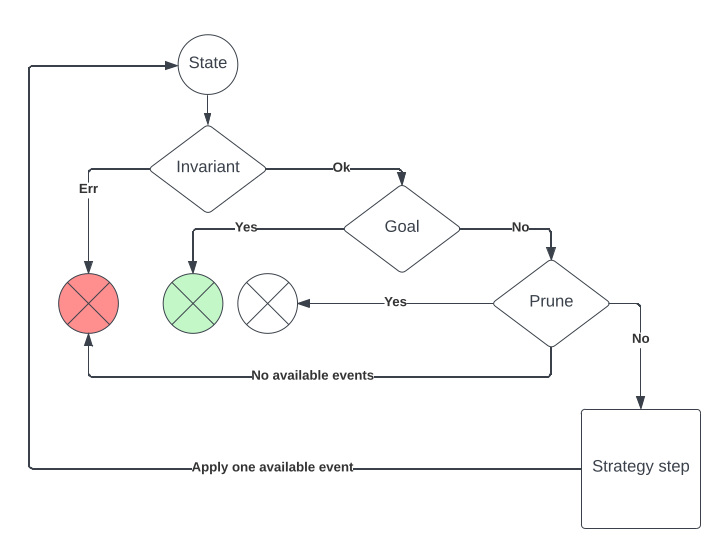
\includegraphics[width=0.5\textwidth]{img/mc_diagram.png}
        \caption{Схема работы \mc\ и разметки состояний}
        \label{mcdiagram}
    \end{center}
\end{figure}

Предикат \goal\ отвечает за определение того, является ли состояние терминальным.
В большинстве случаев \goal\ предполагает, что на все запросы процессы вернут ответы, а в системе больше не останется необработанных событий.

\prune\ отвечает за отсечение различных ветвей исполнения для оптимизации времени работы.
Чаще всего \prune\ используется для отсечения слишком глубоких состояний и добавления в систему дополнительных гарантий.
Например, \prune\ может гарантировать, что даже в сети с отказами сообщение будет доставлено спустя 3 попытки.
Для этого нужно, чтобы \prune\ отсекал все состояния, в которых количество потерянных сообщений больше, чем 2.

\invariant\ проверяет корректность состояния, то есть safety-свойства системы.
Если \invariant\ находит некорректное состояние, \mc\ завершает тест и помечает его как непройденный.

Если \mc\ не нашел ошибок, прошел по всему графу, ни разу не встретил некорректных состояний с помощью \invariant, и все ветви исполнения закончились либо предикатом \prune, либо предикатом \goal, то в таком случае решение считается прошедшим тест (\cref{mcgraph}).



\subsection{Эквивалентные состояния}
\label{visitedstates}

При работе с \mc\ было замечено, что одни и те же состояния могут появляться несколько раз, вследствие различных траекторий.
Например, отправка процессом 1 сообщения процессу 2 и отправка процессом 1 сообщения процессу 3 могут являться независимыми событиями (термин эквивалентности взят из FlyMc \cite{b6}).
Применение таких запросов в различном порядке не изменит финальное состояние системы, но увеличит размер графа состояний.

\begin{figure}
    \begin{center}
        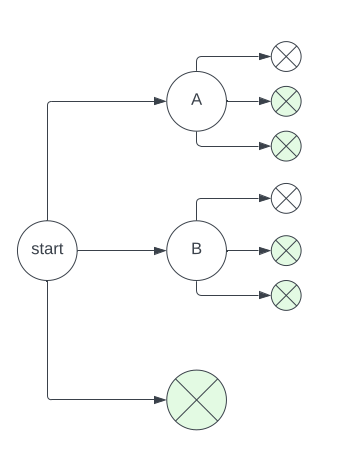
\includegraphics[width=0.3\textwidth]{img/mc_graph_example.png}
        \caption{Пример графа выполнения \mc}
        \label{mcgraph}
    \end{center}
\end{figure}

Для того чтобы не дублировать обход эквивалентных состояний, в DSLab была добавлена сущность \texttt{VisitedStates}.
Эта сущность является хеш-таблицей для проверки того, происходил ли запуск \mc\ из данного состояния ранее.
Поскольку сами по себе состояния системы хранят сериализованное состояние процессов и являются достаточно объемными, то \texttt{VisitedStates} поддерживает два режима: \texttt{Full} и \texttt{Partial}.
Режим \texttt{Full} явно хранит все состояния в хеш-таблице, а \texttt{Partial} разрешает ложно-положительные отсечения, так как хранит только хеши состояний.

Эксперименты показывают, что такой подход заметно уменьшает размер графа состояний (\cref{tab2}).

\begin{table}[htbp]
	\caption{Связь количества состояний в графе для задания ping-pong (\cref{ping_pong_test_1}) с кешированием эквивалентных состояний}
    \begin{center}
    \begin{tabular}{|c|c|c|}
    \hline
     & \textbf{Без кеширования} & \textbf{С кешированием}  \\
    \hline
    \textbf{\# goal} & 677 & 87 \\
    \hline
    \textbf{\# prune} & 1422 & 196 \\
    \hline
    \end{tabular}
    \label{tab2}
    \end{center}
\end{table}

\subsection{Зависимости между событиями}
\label{dependencies}

Новые события появляются в системе, потому что они являются реакцией процесса на какое-то другое событие.
Но эти события не всегда могут быть доступными сразу --- вполне возможно, что одно событие при корректной работе симуляции может произойти только после второго события. 
Контроль доступности событий является важной частью \mc, потому что за счет него проверяется корректность состояния, в котором оказалась система.
За этот контроль отвечают созданные в рамках работы модули \texttt{DependencyResolver} и \texttt{PendingEvents}.

\texttt{PendingEvents} является публичной сущностью, предлагающей контейнер для событий в распределенной системе с возможностью получения списка доступных событий.
\texttt{DependencyResolver} является центральной внутренней компонентой \texttt{PendingEvents}, которая отслеживает доступность событий.

\subsubsection{Отслеживание причинно-следственных связей}
\label{dependenciesdefinition}

В распределенных системах принято связывать события отношением happened-before \cite{b27}.
\texttt{DependencyResolver} должен отслеживать события, которые гарантированно связаны отношением happened-before.

События, которые могут быть упорядочены между процессами --- это срабатывание таймера и доставка сообщения.
При отсутствии гарантий на сеть возможно переупорядочивание любых сообщений между собой.
При отсутствии гарантий на задержки при доставке сообщений возможно переупорядочивание таймеров и сообщений.
Поскольку таймеры находятся на каждом процессе независимо и часы между узлами могут быть не синхронизированы, то возможно переупорядочивание таймеров, находящихся на различных узлах.

Таким образом, \texttt{DependencyResolver} должен отслеживать happened-before для таймеров, находящихся на одном процессе.
Например, если процесс $p$ поставил таймер $t_1$ с длительностью 3, и до истечения $t_1$ поставил таймер $t_2$ длительностью 5, то $t_1$ обязан случиться раньше, чем $t_2$ (\cref{timersgood}).
При этом, если в аналогичной ситуации $t_2$ будет иметь длительность 1, то порядок между $t_1$ и $t_2$ зависит от задержки между временами создания таймеров (\cref{timersbad}).
Поскольку таймеры в асинхронной actor-based модели появляются как реакция на другие события, они могут быть переупорядочены в зависимости от того, какая задержка была между событиями, после которых были поставлены таймеры.
Соответственно, можно гарантировать happened-before $t_1 \to t_2$, только если $\text{created}(t_1) \le \text{created}(t_2)$ и $\text{delay}(t_1) < \text{delay}(t_2)$.
\texttt{DependencyResolver} отслеживает такие зависимости и блокирует таймер $t_2$, если существует $t_1 \to t_2$, и $t_1$ еще не сработал.
Поскольку при обходе графа состояний время является относительной величиной, то \texttt{DependencyResolver} не поддерживает время в явном виде: для сравнения таймеров достаточно хранить $\text{delay}(t_i)$.
Сравнивать $\text{created}(t_i)$ можно с помощью момента добавления таймера в \texttt{DependencyResolver}~--- если таймер $t_1$ был добавлен в систему раньше таймера $t_2$, то
$\text{created}(t_1) < \text{created}(t_2)$. 


\begin{figure}
    \begin{center}
        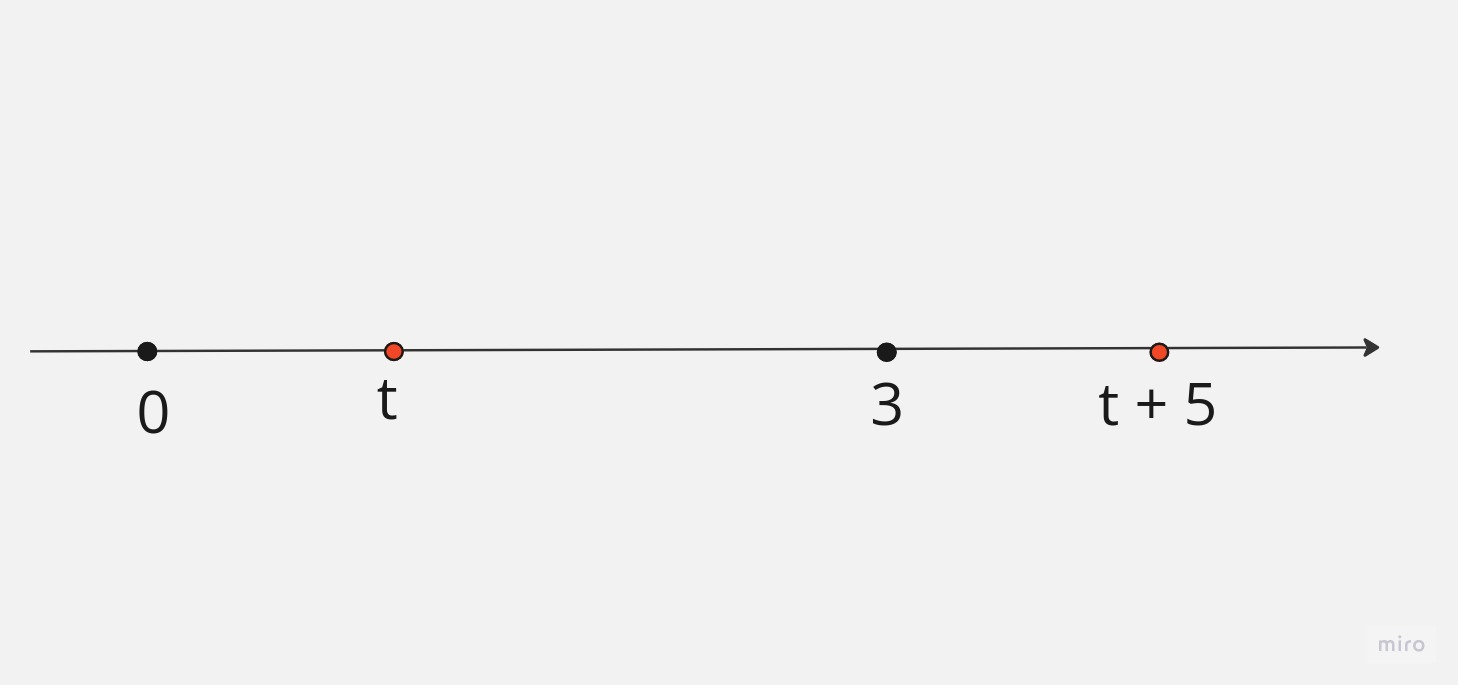
\includegraphics[width=0.5\textwidth]{img/dependency_resolvable.jpg}
        \caption{При заведенном таймере на 3 секунды таймер $t$ с задержкой 5 обязан сработать после момента 3}
        \label{timersgood}
    \end{center}
    \begin{center}
            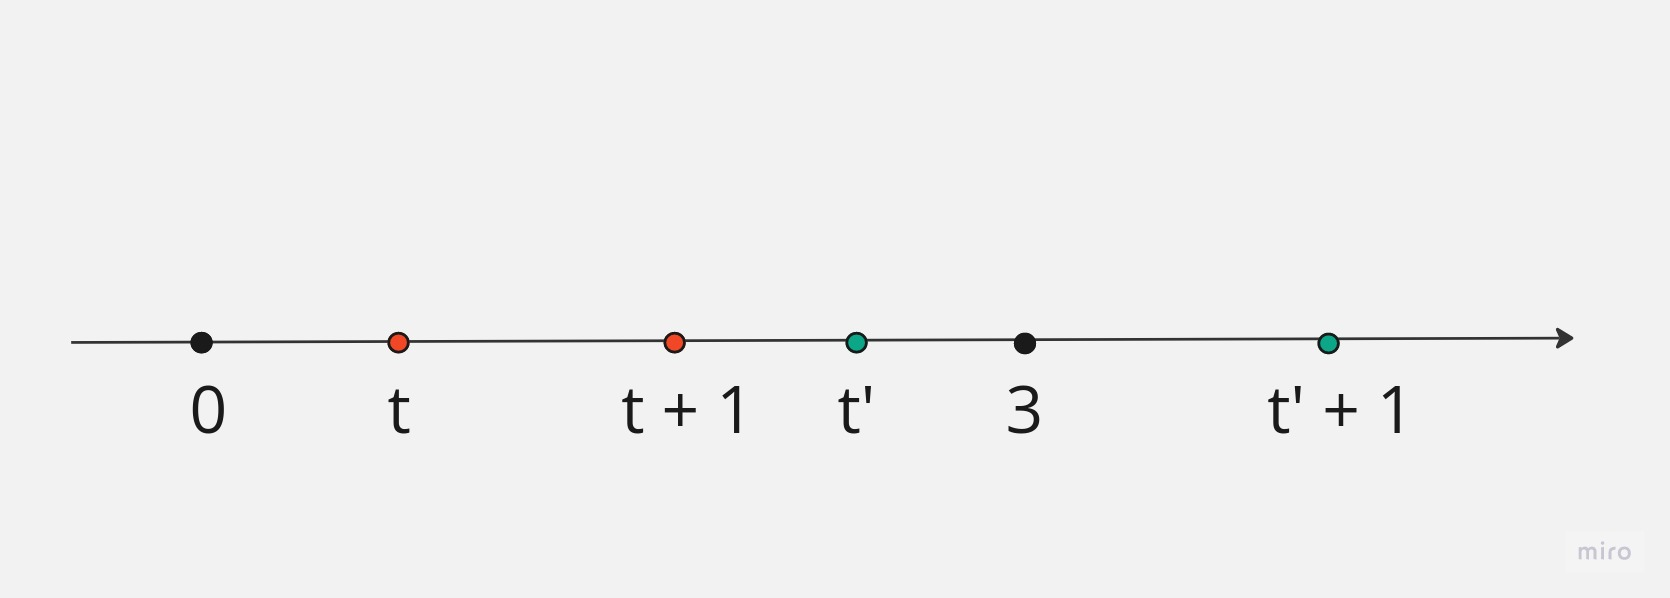
\includegraphics[width=0.5\textwidth]{img/dependency_unresolvable.jpg}
        \caption{При заведенном таймере на 3 секунды таймеры $t$ и $t'$ с задержкой 1 неотличимы, и возможны обе ситуации}
        \label{timersbad}
    \end{center}
\end{figure}


\subsubsection{Обработка группы таймеров}

Дополнительно для оптимизации графа состояний была добавлена сортировка при одновременной работе с набором таймеров.
В ситуациях, где процесс создает несколько таймеров одновременно, ядро \mc\ последовательно добавляет эти таймеры в \texttt{DependencyResolver}.
В главе \ref{dependenciesdefinition} определено, что таймеры $t_1$ и $t_2$ связаны happened-before, если $\text{created}(t_1) \le \text{created}(t_2)$ и $\text{delay}(t_1) < \text{delay}(t_2)$.
При обработке группы таймеров выполняется свойство $\text{created}(t_1) = \text{created}(t_2)$.
Соответственно, обработанные в одной группе таймеры $t_1$ и $t_2$ связаны отношением happened-before, если $\text{delay}(t_1) < \text{delay}(t_2)$.
Поскольку \texttt{DependencyResolver} сравнивает созданные таймеры по моменту их добавления в систему, набор таймеров стоит добавлять в порядке возрастания времени ожидания, чтобы \texttt{DependencyResolver} последовательно связал все таймеры.


\subsubsection{Директивы}

Некоторые события, которые появляются в рамках работы \mc, должны случаться моментально и не зависят друг от друга.
Такими событиями являются отмена таймера и потеря сообщения.
Для них введен специальный тип событий <<директива>>.
Директивам выдается приоритет над другими событиями, поэтому директивы выполняются раньше, чем доставка сообщений или срабатывание таймеров, если есть такой выбор.
Чтобы не перебирать все перестановки имеющихся директив, ядро \mc\ считает не больше одной директивы доступной для выполнения в каждый момент времени.

\subsubsection{Оптимизация отправки дублирующихся сообщений}
\label{equalmessages}

Дополнительно \texttt{DependencyResolver} отвечает за оптимизацию при работе с одинаковыми сообщениями.
В заданиях, где процесс совершает повторную доставку сообщения после определенного времени, два эквивалентных сообщения, оказавшихся в сети, системой воспринимаются как разные.
Но поскольку сообщения эквивалентные, при выборе доступных событий имеет смысл доставлять только первое из них, чтобы уменьшить количество переходов в графе состояний (\cref{tab3}).

\begin{table}[htbp]
    \begin{center}
        \caption{Связь количества состояний в графе для задания ping-pong (\cref{ping_pong_test_1}) с ограничением на отправку дублирующихся сообщений}
        \begin{tabular}{|c|c|c|}
    \hline
     & \textbf{До ограничения} & \textbf{После ограничения}  \\
    \hline
    \textbf{\# goal} & 222 & 87 \\
    \hline
    \textbf{\# prune} & 629 & 196 \\
    \hline
    \end{tabular}
    \label{tab3}
    \end{center}
\end{table}

\subsubsection{Instant Mode}

Было замечено, что комбинация таймеров и сообщений в \mc\ иногда создает траектории, которые потенциально возможны, но не всегда интересны для изучения.
Например, в некоторых задачах требуется определять, вышел ли узел из строя с помощью таймеров.
В таком случае решение студента явно завязано на задержки в сети, и раннее срабатывание таймера приведет систему в состояние, где узел будет помечен отказавшим.
Несмотря на то, что такие состояния теоретически возможны, их тестирование не представляет интереса~--- подобные состояния могут стабилизироваться бесконечно долго, а логика теста, в котором узлы соединены стабильной сетью, чаще всего предполагает, что доставка по умолчанию будет работать корректно.

Разработанный режим Instant Mode предполагает, что сообщения в сети доставляются быстрее, чем срабатывают таймеры.
Таким образом, таймеры в Instant Mode срабатывают, только если все сообщения в сети уже доставлены.
Такой режим оказался полезным в случаях, когда в первую очередь интересно тестирование различных порядков доставки сообщений.

Благодаря этому методу получилось создать исчерпывающий \mc\ для заданий, в которых возможны бесконечные траектории исполнения и рост графа состояний имеет взрывной характер (\cref{MEMBERSHIP}, \cref{KVREPLICATION}).


\subsection{Collect}
\label{collect}

Для того чтобы тестировать систему в специальных состояниях, нужно задать это состояние, как стартовое.
Это не всегда возможно сделать в явном виде, потому что может предполагаться определенное внутреннее состояние системы.

Например, в задании kv-replication (\cref{KVREPLICATION}) существует требование на реализацию sloppy quorum и hinted handoff \cite{b17}.
Для создания состояния, которое проверяет sloppy quorum, сначала требуется нарушение работы системы, а затем ее восстановление.
Подобные случаи удобнее всего тестировать поэтапно.
Первый этап исследует состояния, в котором работа системы нарушена.
После первого этапа происходит восстановления системы.
Второй этап проверяет, что система восстанавливается, то есть достигает ожидаемого корректного состояния.
Можно заметить, что второй этап не может быть запущен сам по себе, потому что внутреннее состояние процессов после отказа хранит информацию о произошедших отказах.
За счет первого этапа происходит заведение системы в требуемое состояние.

Подобный подход для составления тестов в DSLabs называется punctuated search \cite{b1}.
\mc\ в DSLab использует специальный режим \collect\ для punctuated search.
В этом режиме стратегия получает дополнительный предикат, который она использует для сохранения состояний.
Сохраненные состояния из первого графа состояний будут использованы в качестве стартовых во втором графе состояний на измененной системе (\cref{pic3}).

Отличие \collect\ от оригинального punctuated search заключается в том, что \collect\ возвращает множество состояний, и из каждого из них можно запустить \mc.
Это может быть полезно, чтобы протестировать не только работу в произвольном неустойчивом состоянии, но и учесть историю попадания в это состояние.
Например, такой режим успешно используется для тестирования работы при отказе узла в задании <<Надежная упорядоченная рассылка>> (\cref{BROADCAST}), и учитывает момент, в который отключился узел.

Кроме этого, \collect\ можно рассматривать как <<рекурсивный>>, или <<поэтапный>> \mc\ --- когда выполняется \collect\ первого \mc-а, запускается второй этап.
Когда выполняется \collect\ второго этапа, запускается третий, и так далее.
Это оказалось удобно при составлении тестов на kv-хранилища (\cref{KVSHARDING}) --- запросы можно абстрагировать в отдельные методы, и вызывать их друг за другом в режиме \collect.

\begin{figure}
    \begin{center}
        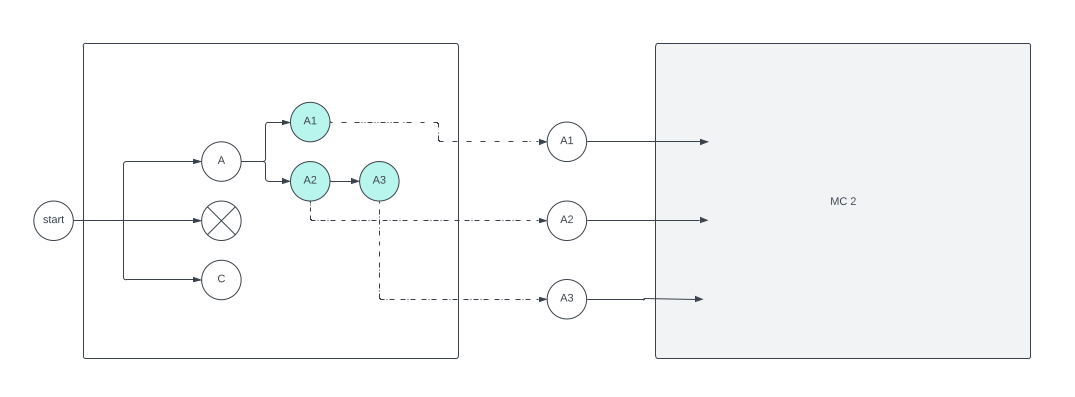
\includegraphics[width=0.9\textwidth]{img/mc_collect.png}
        \caption{Схема работы \mc\ в режиме collect}            
        \label{pic3}
    \end{center}
\end{figure}

\subsection{McSummary}

Для того чтобы интерпретировать результаты работы \mc, имеет смысл получать вердикт, который можно прозрачно интерпретировать.
Недостаточно знать, нарушает решение инварианты или нет --- нужно понимать, как выглядел граф обхода.
Например, помимо проверок свойств safety нужно знать, что не нарушена гарантия liveness.
В таких случаях требуется проверить, что хотя бы один раз сработал \goal.

Для интерпретируемости результатов все предикаты возвращают строковый вердикт, и с помощью \texttt{McSummary}, специальной хеш-таблицы для подсчета статистики, возвращается общий подсчет.
Этот подсчет полезен не только для проверки liveness, но и для оценки размера графа или проведения экспериментов.

\subsection{Выводы}

В рамках работы по переносу ядра \mc\ из dslib в DSLab были созданы дополнительные модули и оптимизации.
Получившееся ядро \mc\ позволяет создавать поэтапное тестирование системы, настраивая режим тестирования, актуальный для задания.
Помимо этого, за счет использования предикатов \goal, \prune\ и \invariant\ стратегии в \mc\ легко кастомизируются под конкретное задание.

Также обновленное ядро \mc\ внимательнее относится к перебору состояний системы.
Во-первых, за счет использования DependencyResolver запрещен перебор невалидных последовательностей событий, которые раньше были возможны.
Во-вторых, был проведен ряд оптимизаций при переборе эквивалентных состояний: отсечение эквивалентных ветвей перебора, оптимизация работы с таймерами.

Добавленный функционал \collect\ помогает готовить гибкие тесты в режиме \mc, создавая поэтапные пайплайны тестирования.
Также был создан режим Instant Mode для удобного тестирования заданий, в которых требуются специальные гарантии на доставку сообщений.

Суммарный объем кода, проделанный в рамках совместного переноса ядра \mc, составляет примерно 1100 строк кода.
Ознакомиться с работой по переносу ядра \mc\ можно по \href{https://github.com/osukhoroslov/dslab/pull/172}{ссылке}.
Вкладом данной работы является несколько компонент: \texttt{McSummary}, \texttt{DependencyResolver}, \texttt{VisitedStates}.
Суммарный объем этих компонент составляет примерно 400 строк программного кода.

Режимы \collect\ и Instant Mode добавлены в рамках улучшения ядра \mc, вместе с небольшими техническими изменениями и оптимизациями.
Общий объем изменений составил примерно 300 строк программного кода и ознакомиться с ним можно по \href{https://github.com/KiK0S/dslab/pull/12}{ссылке}.  

\section{Применение model checking для тестирования решений заданий}
\label{CHAPTER4}

В курсе <<Распределенные системы>> есть 7 заданий на основе dslib --- одна лабораторная работа и 6 домашних заданий.
Каждое задание было перенесено из dslib \cite{b11} в DSLab.
Для перенесенных заданий были подготовлены тесты на \mc.
Тесты были провалидированы на архивном наборе студенческих решений. 

\subsection{Ping-Pong}

В лабораторной работе <<ping-pong>> \cite{b28} требуется написать логику работы процесса-клиента и процесса-сервера.
Процесс-клиент, получая локальное сообщение, шлет сообщение серверу, и ожидает от него ответа.
Предполагается, что в случае ошибок при доставке сообщения, клиент, пользуясь таймером, повторно отправит сообщение серверу.

В тестах к данному заданию система состоит из 2 узлов~--- клиента и сервера.

\begin{table}[htbp]
    \caption{Тесты для ping-pong}
    \begin{center}
    \begin{tabular}{|p{0.2\textwidth}|p{0.2\textwidth}|p{0.2\textwidth}|p{0.3\textwidth}|}
    \hline
    Тест & \goal & \invariant & \prune \\
    \hline
    mc reliable network & Получение 2 сообщений & Имеющиеся ответы верны & Каждый из узлов отправил не больше 4 сообщений  \\
    \hline
    mc unreliable network  & Получение 2 сообщений & Имеющиеся ответы верны & Глубина состояния не больше 7  \\
    \hline
    mc limited drops  & Получение 2 сообщений & Имеющиеся ответы верны & Не больше 3 потерь сообщения, узел отправил не больше 5 сообщений \\
    \hline
    \end{tabular}
    \label{testspingpong}
    \end{center}
\end{table}

\subsubsection{Тест mc\_reliable\_network}
\label{ping_pong_test_1}

Тест симулирует клиента, который отправляет два запроса.
В данном тесте сеть не теряет сообщения, но не дает гарантий на время доставки.

В данном задании технически возможны бесконечные траектории.
Например, возможна ситуация, когда таймер для повторной отправки сообщения всегда срабатывает раньше, чем доставка сообщения.
В таком случае система будет создавать все новые сообщения для доставки по сети, но при этом сообщение так и не будет доставлено.

Для оптимизации размера графа состояний используется \prune, который отсекает состояния, в которых какой-либо из узлов отправил больше 4 сообщений.
Такого отсечения достаточно, чтобы протестировать разные траектории исполнения, необязательно соответствующие идеальным условиям.
При этом такой подход исключает бесконечные цепочки в корректных решениях --- отсечение цепочек из сообщений означает, что возможны только бесконечные цепочки из таймеров, но любое корректное решение не запускает цепочку таймеров, если в результате она не отправит сообщение.
Соответственно, \mc\ может быть выполнен за конечное время вне зависимости от вида решения.


\subsubsection{Тест mc\_unreliable\_network}
\label{ping_pong_test_2}

Тест симулирует клиента, который отправляет два запроса.
В данном тесте сеть может терять сообщения.

В данном задании технически возможны бесконечные траектории.
Так как сеть не гарантирует конечную доставку сообщения, существуют цепочки, где сообщение так и не было доставлено.
Поэтому \mc\ использует отсечение слишком глубоких состояний с помощью \prune.
В качестве глубины для отсечения выбрана глубина 7, так как она больше минимального количества шагов для прохождения теста равно 4 (по 2 сообщения на каждый запрос).
Для глубины 7 обход делается за несколько секунд, и при этом тестируются траектории, в которых помимо базовой доставки сообщений случится потеря сообщения.

\subsubsection{Тест mc\_limited\_drops}
\label{ping_pong_test_3}

Данный тест решает проблему прошлого теста (\cref{ping_pong_test_2}).
Бесконечные цепочки возникают, когда происходит бесконечная потеря сообщений.
Для того чтобы сделать исчерпывающий \mc, достаточно поставить лимит на количество потерянных сообщений, и свести тест к уже имеющейся модели (\cref{ping_pong_test_1}).
Это значит, что дополнительно понадобится отсечение на количество отправленных сообщений, которое автоматически повлечет за собой отсечение по количеству таймеров.

Для оптимизации размера графа состояний используется \prune, который отсекает состояния с более чем 3 потерями сообщений.

\subsubsection{Результаты}

Для данного задания отсутствует архив студенческих решений, так что тестирование проводилось на 2 авторских решениях (одном корректном и одном некорректном).
Результаты тестирования приведены в \cref{tab4}.

Тесты \mc\ (\cref{testspingpong}) нашли гарантию, на которую неявно полагалось авторское решение, но которой не было дано в условии.
Авторское решение предполагало, что новый запрос от клиента может прийти только тогда, когда система ответила на предыдущий запрос.
\mc\ привел систему в состояние, когда два запроса в ней существовали одновременно, и в таком случае в некоторых траекториях исполнения решение получало ошибку выполнения.

Таким образом, было добавлено третье решение, исправляющее ошибку в авторском решении.

\begin{table}[htbp]
    \caption{Тесты model checking в задании Ping-Pong}
    \begin{center}
    \begin{tabular}{|c|c|c|}
    \hline
    \textbf{Тест} & \textbf{\# accepted} & \textbf{\# failed}  \\
    \hline
    mc\_reliable\_network & 2 & 1 \\
    \hline
    mc\_unreliable\_network & 1 & 2 \\
    \hline
    mc\_limited\_drops & 1 &  2 \\
    \hline

    \end{tabular}
    \label{tab4}
    \end{center}
\end{table}


\subsection{Гарантии доставки}
\label{GUARANTEES}

В задании <<Гарантии доставки>> \cite{b13} требуется реализовать доставку сообщений с соблюдением различных гарантий:
\begin{enumerate}
\item At Least Once: каждое отправленное сообщение будет получено хотя бы один раз.
\item At Most Once: каждое отправленное сообщение будет получено не более одного раза.
\item Exactly Once: каждое отправленное сообщение будет получено ровно один раз.
\item Exactly Once Ordered: то же самое, что и Exactly Once, но сообщения должны быть доставлены в соответствии с порядком отправки.
\end{enumerate}

В тестах к данному заданию система состоит из 2 узлов~--- отправителя и получателя.
Доставку требуется реализовывать между процессами \texttt{sender} и \texttt{receiver}, расположенных на соответствующих узлах.
Предполагается, что решение реализует каждую из гарантий по отдельности, с помощью комбинации механизмов повторной доставки (необходимый для At Least Once), отсеивания дубликатов (необходимый для At Most Once), и упорядочивания сообщений с помощью временных меток (для Ordered-гарантии). 


\begin{table}[htbp]
    \caption{Тесты для задания <<Гарантии доставки>>}
    \begin{center}
    \begin{tabular}{|p{0.2\textwidth}|p{0.2\textwidth}|p{0.2\textwidth}|p{0.3\textwidth}|}
    \hline
    Запуск \mc & \goal & \invariant & \prune \\
    \hline
    mc reliable network & Доставка 2 сообщений & Имеющиеся ответы верны & Узел отправляет не более 4 сообщений и ставит не более 4 таймеров  \\
    \hline
    mc unreliable network  &  Доставка 2 сообщений & Имеющиеся ответы верны & Глубина состояния не больше 5  \\
    \hline
    mc limited drops  & Доставка 2 сообщений & Имеющиеся ответы верны & Не больше 3 потерь сообщений, узел отправляет не более 4 сообщений и ставит не более 4 таймеров \\
    \hline
    \end{tabular}
    \label{testsguarantees}
    \end{center}
\end{table}

\subsubsection{Тест mc\_reliable\_network}
\label{guarantees_test_1}

Тест симулирует клиента, который отправляет два запроса.
В данном тесте сеть не теряет сообщения, но не дает гарантий на время доставки.

В данном задании технически возможны бесконечные траектории.
Например, возможна ситуация, когда таймер для повторной отправки сообщения срабатывает раньше, чем доставка сообщения.


Для оптимизации размера графа состояний используется \prune, который выполняет отсечение по количеству отправленных с каждого узла сообщений и заведенных таймеров.
Такой подход исключает бесконечные цепочки в корректных решениях. 

\subsubsection{Тест mc\_unreliable\_network}
\label{guarantees_test_2}

Тест симулирует клиента, который отправляет два запроса.
В отличие от прошлого теста (\cref{guarantees_test_1}), данном тесте сеть может терять сообщения.

В данном задании технически возможны бесконечные траектории.
Так как сеть не гарантирует конечную доставку сообщения, существуют цепочки, где сообщение так и не было доставлено.
Поэтому \mc\ использует отсечение по глубине обхода.
Выбрана глубина обхода 5 для баланса между временем выполнения теста и найденными ошибками.
Можно заметить, что для доставки двух сообщения достаточно 2 сообщений в сети.
Запас в 3 дополнительных события означает, что также будут проверены safety-свойства в состояниях, где успели дополнительно сработать таймеры, произойти дополнительные доставки сообщений, потери сообщений или доставка сообщений-подтверждений от получателя.

\subsubsection{Тест mc\_limited\_drops}
\label{guarantees_test_3}

Данный тест решает проблему прошлого теста (\cref{guarantees_test_2}).
Бесконечные цепочки возникают, когда происходит бесконечная потеря сообщений.
Для того чтобы сделать исчерпывающий \mc, достаточно поставить лимит на количество потерянных сообщений, и свести тест к уже имеющейся модели (\cref{guarantees_test_1}).

Для оптимизации размера графа состояний используется \prune, который отсекает состояния с большим количеством  потерянных сообщений, отправленных сообщений и заведенных таймеров.
Также \prune\ отсекает состояния с более чем 3 потерями сообщений.

Такой тест оказывается полным, и тестирует большое количество различных траекторий и случаев при выполнении теста.


\subsubsection{Результаты}

Результаты тестирования приведены в \cref{tab5}.

При тестировании (\cref{testsguarantees}) архивных студенческих решений были найдены следующие ошибки:
\begin{enumerate}
    \item Решение делало отложенную очистку кеша и забывало факт доставки сообщения, за счет чего доставка одного и того же сообщения могла случиться несколько раз.
Такая ошибка встретилась в двух решениях.
    \item Решение на гарантию At Most Once при срабатывании таймера могло проигнорировать сообщение $X$ как полученное ранее, даже если $X$ доставлено впервые.
Несмотря на то, что формально это At Most Once, в задаче явно оговорено, что при отсутствии отказов сети решение должно доставлять запросы.
\end{enumerate} 

Можно заметить, что в этом задании \mc\ в основном находит ошибки в решениях, которые полагались на таймеры, и преждевременное срабатывание таймера могло нарушить инварианты.
Такие решения слишком сильно опирались на свойства сети (а именно задержку при доставке), за счет чего могут вести себя некорректно, если задержка изменится.

\begin{table}[htbp]
    \caption{Результаты тестирования студенческих решений в задании <<Гарантии доставки>>. Рядом с числом ошибочных решений в скобках указано, сколько из них ранее были оценены на максимально возможный балл. }
    \begin{center}
    \begin{tabular}{|c|c|c|}
    \hline
    \textbf{Тест [гарантия]} & \textbf{\# accepted} & \textbf{\# failed}  \\
    \hline
    mc\_reliable\_network [AMO]  & 51 & 39 (1) \\
    mc\_reliable\_network [ALO] & 52 & 38 (0) \\
    mc\_reliable\_network [EO] & 49 & 41 (2) \\
    mc\_reliable\_network [EOO] & 48 & 42 (0) \\
    \hline
    mc\_unreliable\_network [AMO] & 51 & 39 (1) \\
    mc\_unreliable\_network [ALO] & 52 & 38 (0) \\
    mc\_unreliable\_network [EO] & 49 & 41 (2) \\
    mc\_unreliable\_network [EOO] & 48 & 42 (0) \\
    \hline
    mc\_limited\_drops [AMO] & 51 &  39 (1) \\
    mc\_limited\_drops [ALO] & 51 &  39 (0) \\
    mc\_limited\_drops [EO] & 49 &  41 (2)\\
    mc\_limited\_drops [EOO] & 46 &  44 (0)\\
    \hline

    \end{tabular}
    \label{tab5}
    \end{center}
\end{table}

\subsection{Надежная упорядоченная рассылка}
\label{BROADCAST}
В задании <<Надежная упорядоченная рассылка>> \cite{b14} требуется доставить сообщение большинству узлов в кластере.
Узлы могут отказывать, но гарантируется, что после отказа они не восстанавливаются до конца теста.
Доставка сообщений надежная.
Таким образом, единственные сбои могут возникнуть из-за того, что узел вышел из строя.
Узлы, которые не отказали до конца теста, называются корректными.
Гарантируется, что более половины узлов в системе корректны.

К решению предлагаются следующие обязательные требования:

\begin{enumerate}
\item No Creation: каждое принятое сообщение должно быть предварительно отправлено 
\item No Duplication: каждое принятое сообщение должно быть доставлено единожды
\item Validity: если корректный узел $n$ отправил другому узлу сообщение $m$, то $n$ обязательно доставит $m$
\item Uniform agreement: если узел $n$ (необязательно корректный) принял сообщение $m$, то $m$ в конечном счете будет принято на каждом корректном узле.
\end{enumerate}

Предполагается, что процессы рассылают сообщения всем остальным процессам в сети, и собирают информацию о том, набралось ли большинство процессов, готовых доставить сообщение.

В тестах к данному заданию система состоит из 3 узлов.
Таким образом, гарантируется корректность хотя бы 2 узлов.


\begin{table}[htbp]
    \caption{Тест mc\_normal}
    \begin{center}
    \begin{tabular}{|p{0.15\textwidth}|p{0.2\textwidth}|p{0.2\textwidth}|p{0.2\textwidth}|p{0.2\textwidth} |}
    \hline
    Этап & \goal & \invariant & \prune & \collect \\
    \hline
    Доставка & Сообщение доставлено всеми корректными узлами & Соблюден формат доставленных клиенту сообщений & Каждый узел отправил не больше 2 сообщений, эквивалентные состояния игнорируются, глубина не более 10 & - \\
    \hline    
    \end{tabular}
    \label{testsbroadcast_1}
    \end{center}
\end{table}

\subsubsection{Тест mc\_normal}

Тест соответствует нормальной рассылке сообщения, когда отказов не существует.
Теоретически, в данном задании не должно возникать бесконечных цепочек.
На практике оказалось, что обход может занимать несколько минут даже для 3 узлов.
Это связано с тем, что типичное решение рассылает сообщения по логике <<от всех всем>>.
Таким образом, возможны перестановки сообщений, которые увеличивают размер графа состояний экспоненциально.

В данном задании важно сделать правильные отсечения с помощью \prune.
В тесте, помимо ограничений на состояние, делается проверка состояний на <<эквивалентность>>.
Предполагается, что узлы одинаковы между собой, поэтому любая перестановка узлов не меняет состояние.
По этой причине отсечение проверяет, что порядок, в котором узлы "встречаются" в последовательности, соответствуют тривиальной перестановке узлов.

\subsubsection{Тест mc\_sender\_crash}

\begin{table}[htbp]
    \caption{Тест mc\_sender\_crash}
    \begin{center}
    \begin{tabular}{|p{0.15\textwidth}|p{0.2\textwidth}|p{0.2\textwidth}|p{0.2\textwidth}|p{0.2\textwidth} |}
    \hline
    Этап & \goal & \invariant & \prune & \collect \\
    \hline
    До отказа & Сообщение доставлено всеми корректными узлами & Соблюден формат доставленных клиенту сообщений & Глубина не более 4 & Хотя бы один узел получил сообщение \\
    \hline
    Выведение из строя отправителя & - & - & - & -\\
    \hline
    Доставка после отказа  & Сообщение доставлено всеми корректными узлами & Соблюден формат доставленных клиенту сообщений & Каждый узел отправил не больше 4 сообщений, эквивалентные состояния игнорируются, глубина не более 6 & - \\
    \hline
    \end{tabular}
    \label{testsbroadcast_2}
    \end{center}
\end{table}


Тест предполагает, что по ходу выполнения программы узел-отправитель сообщения откажет.
Событие отказа узла является достаточно сложным для моделирования, потому что, например, узел отправителя сообщения не может отказать, пока он не отправил сообщение хотя бы одному корректному узлу.
Для того чтобы правильно отслеживать такие события, используется механизм punctuated search.
С помощью режима \collect\ делается первый запуск \mc, который собирает все состояния, в которых отправитель отправил сообщение хотя бы одному другому узлу.

После этого для каждого собранного состояния выводится из строя процесс-отправитель, и запускается новый \mc, который проверяет, что даже с учетом отказавшего отправителя сообщение доставится на большинство узлов.
Таким образом, в рамках этого теста происходит много разных запусков \mc, которые делают полный обход графа состояний вместе с punctuated search, что делает более точное тестирование, чем оригинальный punctuated search в DSLabs \cite{b1}.

\subsubsection{Результаты}

Результаты тестирования приведены в \cref{tab6}.

При тестировании (\cref{testsbroadcast_1} и \ref{testsbroadcast_2}) архивных студенческих решений были найдены следующие ошибки:
\begin{enumerate}
    \item Решение делало некорректную инициализацию ресурсов, которая опиралось на то, что сообщение от процесса самому себе будет доставлено раньше, чем случится коммуникация между двумя различными процессами.
    \item Решение некорректно проверяло необходимость локальной доставки сообщения. Счетчик инициализировался таким образом, что в системе из трех узлов решение пропускало момент, когда счетчик набирал кворум, за счет чего сообщение не доставлялось.
    \item 7 решений неэффективно использовали сеть --- отдельно производили массовую рассылку целевого сообщения и отдельно массово рассылали факт получения данного сообщения, хотя данные сообщения можно объединить и снизить нагрузку на сеть в 2 раза.
\end{enumerate} 

\begin{table}[htbp]
    \caption{Результаты тестирования студенческих решений в задании <<Надежная упорядоченная рассылка>>. Рядом с числом ошибочных решений в скобках указано, сколько из них ранее были оценены на максимально возможный балл. }
    \begin{center}
    \begin{tabular}{|c|c|c|}
    \hline
    \textbf{Тест} & \textbf{\# accepted} & \textbf{\# failed}  \\
    \hline
    mc\_normal  & 69 & 11 (10) \\
    \hline
    mc\_sender\_crash & 69 & 11 (10) \\
    \hline

    \end{tabular}
    \label{tab6}
    \end{center}
\end{table}

\subsection{Group membership}
\label{MEMBERSHIP}

В задании <<Group membership>> \cite{b15} требуется реализовать детектор отказов и распределенный сервис для отслеживания состава группы на его основе.
Узлы, обмениваясь сообщениями с другими узлами, поддерживают актуальную информацию о связанных с ними узлами в группе.
Предполагается, что узлы обмениваются сообщениями, и помечают узел как отказавший при отсутствии ответа.

В тестах к данному заданию система состоит из 2 узлов.
При корректной работе сети оба узла должны находиться в составе одной группы, а при отказах системы каждый узел должен выделяться в собственную группу.

В тестах используется Instant Mode, так как таймеры определяют отказавшие узлы.
В случае перестановок таймеров с сообщениями в случайном порядке, решение не сможет стабилизировать статус каждого узла.
В Instant режиме сообщения имеют больший приоритет, чем таймеры, поэтому доставка сообщения и получение ответа будут происходить до срабатывания timeout-таймера.


\begin{table}[htbp]
    \caption{Тесты для задания <<Group membership>>}
    \begin{center}
    \begin{tabular}{|p{0.1\textwidth}|p{0.15\textwidth}|p{0.2\textwidth}|p{0.2\textwidth}|p{0.2\textwidth} |}
    \hline
    Запуск \mc & \goal & \invariant & \prune & \collect \\
    \hline
    local answer & Получен ответ на запрос & Ответ корректный, глубина обхода не больше 5 & - & - \\
    \hline
    normal 1  & Больше нет доступных событий & - & Процесс запустил не более 5 таймеров, глубина обхода не больше 15, каждое событие не повторяется больше, чем дважды & Все узлы получили по 3+ сообщения, глубина обхода больше 15 или кончились доступные события \\
    \hline
    normal 2 & Получены ответ на запросы & Ответы корректные, глубина обхода не больше 2 & - & - \\
    \hline
    \end{tabular}
    \label{testmembership}
    \end{center}
\end{table}

\subsubsection{Тест mc\_local\_answer}

Данный тест с помощью \mc\ проверяет, что решение отвечает на локальный запрос GET\_MEMBERS моментально.

Для этого \invariant\ отсекает все состояния на глубине 2 и больше.

Этот тест был использован для двух целей:
\begin{enumerate}
    \item Для других тестов в данном задании был полезен запуск \mc, который проверяет ответ каждого узла на локальный запрос.
Такая проверка позволяет делать остальные тесты на \mc\ более эффективно.
    \item Благодаря тестированию архивных решений на этом тесте можно было сделать анализ того, насколько предположение о локальности ответов на запрос верно для всех решений.
Тесты показали, что все решения отвечают на запрос состава группы локальным сообщением, несмотря на то, что изначальные требования к реализации не запрещают делать дополнительные запросы.
\end{enumerate}

\subsubsection{Тест mc\_normal}

Данный тест проверяет стабилизацию состава группы из двух узлов.
Он состоит из двух шагов, каждый из которых является запуском \mc:
\begin{enumerate}
    \item Сначала собираются состояния, соответствующие различным траекториям исполнения.
Предполагается, что \collect\ должен собрать состояния, в которых система уже должна была стабилизировать состав группы.
Для этого каждый узел должен получить достаточное сообщение узлов от соседей, достаточно 3 сообщений.
Также если решение создает невалидные траектории исполнения, \collect\ должен их отлавливать через слишком большую глубину состояния или отсутствие доступных событий.
Для того чтобы ограничить обход графа состояний, \prune\ ограничивает количество таймеров (ограничение в 5 таймеров дает запас для исследования различных нетривиальных траекторий).
Помимо ограничения на таймеры есть ограничение на дубликаты событий.
Предполагается, что когда одно и то же событие происходит повторно (например, двойная доставка одного и того же сообщения), возможны ошибки при обработке повторного применения события.
При этом ошибки для состояний, в которых событие произошло больше двух раз, и не проявляющееся при первом дублировании события, маловероятны.
Такое отсечение помогает заметно уменьшить размер графа состояний, при этом все еще проверяя корректность решений.
Также \prune\ ограничивает общую глубину для конечного размера графа состояний.
    \item В каждом собранном состоянии проверяется состав группы с помощью локальных запросов.
\end{enumerate}

% В первом запуске \mc\ \invariant\ и \goal\ игнорируются.
% \collect\ собирает состояния, в которых каждый процесс получил хотя бы по два сообщения.
% Также \collect\ собирает состояния, в которых исчерпаны все возможные переходы.
% \prune\ отсекает состояния, в которых сработало более 5 таймеров на каком-либо из узлов, а также состояния с глубиной больше 15.

% На втором запуске \mc\ происходит проверка, что состав группы стабилизировался.
% \invariant\ проверяет корректность ответов и отсутствие глубины больше 1.

\subsubsection{Тест mc\_partition\_recovery}

Данный тест проверяет стабилизацию группы, затем путем разделения сети делит группу на две части, а затем собирает ее обратно, восстанавливая сеть.
Соответственно, данный тест предполагает шесть последовательных запусков model checking:

\begin{enumerate}
    \item Сначала собираются состояния, соответствующие различным траекториям исполнения
    \item В каждом собранном состоянии проверяется состав группы с помощью локальных запросов.
    \item Разделяется сеть и собираются состояния, соответствующие различным траекториям исполнения
    \item В каждом собранном состоянии проверяется состав группы с помощью локальных запросов.
    \item Сеть возвращается в нормальный режим и собираются состояния, соответствующие различным траекториям исполнения
    \item В каждом собранном состоянии проверяется состав группы с помощью локальных запросов.
\end{enumerate}


\begin{table}[htbp]
    \caption{Описание теста mc\_partition\_recovery}
    \begin{center}
    \begin{tabular}{|p{0.1\textwidth}|p{0.15\textwidth}|p{0.2\textwidth}|p{0.3\textwidth}|p{0.2\textwidth} |}
    \hline
    Запуск \mc & \goal & \invariant & \prune & \collect \\
    \hline
    1  & Больше нет доступных событий & - & Процесс запустил не более 5 таймеров, глубина обхода не больше 15, каждое событие не повторяется больше, чем дважды & Все узлы получили по 3+ сообщения, глубина обхода больше 15 или кончились доступные события \\
    \hline
    2 & Получены ответ на запросы & Ответы корректные, глубина обхода не больше 2 & - & Получены правильные ответы на запросы \\
    \hline
    3 & Глубина больше 30 или нет доступных событий & - & Не больше 3 повторений одного события, не больше 5 таймеров на процесс и не больше 8 в сумме, не больше 10 таймеов на процесс и не больше 18 в сумме  & Глубина больше 30 или нет доступных событий \\
    \hline
    4 & Получены ответ на запросы & Ответы корректные, глубина обхода не больше 2 & - & Получены правильные ответы на запросы \\
    \hline
    5  & Больше нет доступных событий & - & Процесс запустил не более 5 таймеров, глубина обхода не больше 15, каждое событие не повторяется больше, чем дважды & Все узлы получили по 3+ сообщения, глубина обхода больше 15 или кончились доступные события \\
    \hline
    6 & Получены ответ на запросы & Ответы корректные, глубина обхода не больше 2 & - & - \\
    \hline

    \end{tabular}
    \label{testmembershiprecovery}
    \end{center}
\end{table}




% При работе над тестом было выявлено,

% В первом запуске model checking \invariant\ и \goal\ игнорируются.
% \collect\ собирает состояния, в которых каждый процесс получил хотя бы по два сообщения.
% Также \collect\ собирает состояния, в которых исчерпаны все возможные переходы.
% \prune\ отсекает состояния, в которых сработало более 5 таймеров на каком-либо из узлов, а также состояния с глубиной больше 15.

% На втором запуске model checking происходит проверка, что состав группы стабилизировался.
% \invariant\ проверяет корректность ответов и отсутствие глубины больше 1.


% В третьем запуске model checking \invariant\ и \goal\ игнорируются.
% \collect\ собирает состояния, в которых каждый процесс попробовал отправить хотя бы по два сообщения.
% Также \collect\ собирает состояния, в которых исчерпаны все возможные переходы.
% \prune\ отсекает состояния, в которых глубина больше 13.

% На четвертом запуске model checking происходит проверка, что состав группы стабилизировался.
% \invariant\ проверяет корректность ответов и отсутствие глубины больше 1.




% В пятом запуске model checking \invariant\ и \goal\ игнорируются.
% \collect\ собирает состояния, в которых каждый процесс получил хотя бы по два сообщения.
% Также \collect\ собирает состояния, в которых исчерпаны все возможные переходы.
% \prune\ отсекает состояния, в которых сработало более 5 таймеров на каком-либо из узлов, а также состояния с глубиной больше 15.

% На шестом запуске model checking происходит проверка, что состав группы стабилизировался.
% \invariant\ проверяет корректность ответов и отсутствие глубины больше 1.


\subsubsection{Результаты}

Результаты тестирования приведены в \cref{tab7}.

При тестировании (\cref{testmembership}) архивных студенческих решений были найдены следующие ошибки:
\begin{enumerate}
    \item Решение заводило несколько различных таймеров: таймер HEARTBEAT запускал проверку соседних узлов на наличие активного соединения путем рассылки сообщений, таймер TIMEOUT отсекал не успевавшие ответить узлы как отказавшие.
Существует промежуток времени, в который может сработать таймер TIMEOUT, потому что ответ на HEARTBEAT еще не был доставлен.
В таком случае решение могло ложно записать узел в отказавшие.
В списке отказавших узлов для процесса $X$ мог быть даже узел с процессом $X$.
При этом данный баг может воспроизводиться много раз и нарушает требование на liveness решения.
    \item Было найдено неэффективное решение, которое делает в два раза больше отправок сообщений по сети, чем требуется.
Решение рассылало состав группы только доступным соседям, а доступных соседей определяло с помощью PING-запросов.
Неоптимальность заключается в том, что есть возможность сразу рассылать узлам состав группы, и определять доступных по наличию ответа на запрос.
\end{enumerate} 


Тест mc\_partition\_recovery (\cref{testmembershiprecovery}) был подготовлен и протестирован вручную на отдельных студенческих решениях, но протокол взаимодействия процесса и тестирующей системы не обладает достаточным функционалом для автоматического тестирования всех решений в архиве.
Это связано с тем, что студенческое решение определяет отказ узла после срабатывания таймера с произвольным именем.
За счет того, что решение задачи предполагает заведение нескольких таймеров, нельзя сделать реализацию \collect, которая бы могла собрать состояния, уже обнаружившие отказ узла.
Решить данную проблему можно путем отправки локального сообщения в систему внутри вызова \collect, но текущее ядро \mc\ не имеет такой возможности и соответствующие доработки достаточно сильно изменят структуру ядра \mc.
Альтернативно данную проблему можно решить изменением протокола взаимодействия решения и тестирующей системы.
В таком случае решение будет отправлять локальный запрос на каждое изменение состава группы и \collect\ сможет по информации в логе понять, был ли определен отказ узла.

\begin{table}[htbp]
    \caption{Результаты тестирования студенческих решений в задании <<Group membership>>. Рядом с числом ошибочных решений в скобках указано, сколько из них ранее были оценены на максимально возможный балл. }
    \begin{center}
    \begin{tabular}{|c|c|c|}
    \hline
    \textbf{Тест} & \textbf{\# accepted} & \textbf{\# failed}  \\
    \hline
    mc\_local\_answer  & 76 & 0 (0) \\
    \hline
    mc\_normal  & 28 & 48 (2) \\
    \hline
    mc\_partition\_recovery & - & -  \\
    \hline

    \end{tabular}
    \label{tab7}
    \end{center}
\end{table}


\subsection{Распределенное key-value хранилище с шардингом}
\label{KVSHARDING}


В задании <<Распределенное key-value хранилище с шардингом>> \cite{b16} требуется сделать kv-хранилище, которое хранит данные распределенно на разных узлах, и в случае отказа совершает перебалансировку.
В этом задании отказы симулируются через запросы добавления и удаления узлов.
Таким образом, можно считать, что система всегда доставляет сообщения, и отказов нет, есть только перебалансировка ключей.

В тестах к данному заданию система состоит из 3 узлов, каждый из которых отвечает на свою часть хранилища.

В этом задании важно обеспечить последовательные запросы на добавление и получение значений по ключу.
Ожидается, что решение пересылает запрос на узел, отвечающий за хранение конкретного ключа.
За счет этого граф исполнения для корректного решения остается компактным даже при большом количестве последовательных запросов --- финальное состояние системы после ответа на запрос всегда одинаково.

Чтобы находить неэффективные решения, \invariant\ явно запрещает слишком длинные траектории исполнения.
Предполагается, что запросы get, put, delete требуют 2 события~---- пересылку запроса на шард и получение ответа с шарда.
Для перебалансировки возможно большее количество событий~--- узлы могут отправить по сообщению на каждый другой узел.
Для системы из 3 узлов это соответствует 6 сообщениям.
Таким образом, можно считать, что любому решению должно хватить 10 шагов до конца обработки запроса.


\begin{table}[htbp]
    \caption{Тесты для задания <<Распределенное key-value хранилище с шардингом>>}
    \begin{center}
    \begin{tabular}{|p{0.15\textwidth}|p{0.3\textwidth}|p{0.3\textwidth}|p{0.1\textwidth}|p{0.1\textwidth} |}
    \hline
    Запуск \mc & \goal & \invariant & \prune & \collect \\
    \hline
    normal 1: get & Получен ответ и доступные события кончились & Ответ соответствует ожидаемому и глубина не более 10 & - & Получен ответ \\
    normal 2: put & Получен ответ и доступные события кончились & Ответ соответствует ожидаемому и глубина не более 10 & - & Получен ответ \\
    normal 3: get & Получен ответ и доступные события кончились & Ответ соответствует ожидаемому и глубина не более 10 & - & Получен ответ \\
    normal 4: delete & Получен ответ и доступные события кончились & Ответ соответствует ожидаемому и глубина не более 10 & - & Получен ответ \\
    normal 5: get & Получен ответ и доступные события кончились & Ответ соответствует ожидаемому и глубина не более 10 & - & Получен ответ \\
    \hline
    rebalance 1 (x40): put & Получен ответ и доступные события кончились & Ответ соответствует ожидаемому и глубина не более 10 & - & Получен ответ \\
    rebalance 2: node removed & Все узлы обработали запрос и доступные события кончились & Ответы соответствуют ожидаемым и глубина не более 10 & - & Получены ответы \\
    rebalance 3 (x40): get & Получен ответ и доступные события кончились & Ответ соответствует ожидаемому и глубина не более 10 & - & Получен ответ \\
    \hline
    \end{tabular}
    \label{testskvsharding}
    \end{center}
\end{table}

\subsubsection{Тест mc\_normal}

С помощью \mc\ были реализованы примитивы для проверки работы каждого запроса на корректность.
Это означает, что для каждого типа запросов Get, Put, Delete были сделаны функции, которые содержали в себе проверку конкретного запроса с помощью \mc.
Режим \collect\ в данном случае собирает все возможные траектории выполнения первого запроса, и из каждого из них начинал выполнение второго запроса.
Полученные состояния после второго запроса используются, чтобы начать третий запрос и так далее.

Тест mc\_normal последовательно через данные примитивы сделал последовательность запросов, чтобы проверить логику ответа на запросы.
Последовательность запросов соответствует базовому тесту из стандартного набора.

\subsubsection{Тест mc\_rebalance}

Данный тест использует запрос Node removed, чтобы имитировать выход узла из сети.
Обработка такого запроса в тестах реализован с помощью \mc\ аналогично остальным запросам.

В тесте сначала создается 40 записей с помощью последовательных put-запросов.
Затем один из узлов отключается и система стабилизируется с помощью \mc.
После стабилизации происходит 40 запросов на чтение.
Ожидается, что после стабилизации все чтения происходят успешно.



\subsubsection{Результаты}

Результаты тестирования приведены в \cref{tab8}.

Корректное решение на тестах в этом задании всегда следует по одной траектории, потому что все альтернативные траектории отличаются перестановкой независимых сообщений и считаются эквивалентными.
Таким образом, в этом задании \mc\ помогает не только искать ошибки, но и проверять, соответствует ли граф состояний ожидаемой структуре.

Тесты на \mc\ (\cref{testskvsharding}) не отловили в этой задаче новых ошибок в студенческих решениях, но нашли существовавшие ранее ошибки.
Например, те решения, которые делали неэффективную перебалансировку и отправляли больше одного сообщений между двумя репликами, получали ошибку из-за достижения слишком большой глубины обхода.

\begin{table}[htbp]
    \caption{Результаты тестирования студенческих решений в задании <<Распределенное key-value хранилище с шардингом>>. Рядом с числом ошибочных решений в скобках указано, сколько из них ранее были оценены на максимально возможный балл. }
    \begin{center}
    \begin{tabular}{|c|c|c|}
    \hline
    \textbf{Тест} & \textbf{\# accepted} & \textbf{\# failed} \\
    \hline
    mc\_normal  & 74 & 0 (0) \\
    \hline
    mc\_rebalance  & 24 & 50 (0) \\
    \hline
    \end{tabular}
    \label{tab8}
    \end{center}
\end{table}

\subsection{Распределенное key-value хранилище с репликацией}
\label{KVREPLICATION}

В задании kv-replication нужно реализовать kv-хранилище, которое хранит данные с высокой доступностью.
Требуется использовать кворум, чтобы данные писались хотя бы на W реплик, а читались хотя бы с R реплик.
В данном задании используется 3 реплики, поэтому верно выражение $W+R>3$.
В такой конфигурации можно получить корректный ответ на запрос даже при отказе одного узла.
Задание дополнительно требует реализовать механизмы sloppy quorum и hinted handoff, соответствующие механизмам из Amazon Dynamo \cite{b29}, которые позволяют ответить на запрос даже при недостатке активных реплик, и восстановить корректное состояние системы после восстановления соединения. 

В тестах к данному заданию система состоит из 4 узлов.
За счет этого для каждого ключа в системе есть 3 реплики, которые должны хранить значение для этого ключа, а также одна дополнительная вершина, которая может использоваться в качестве теневой реплики при отказах в сети.


\subsubsection{Тест mc\_normal}
\label{kvreplication_test_1}

\begin{table}[htbp]
    \caption{Тест mc\_normal}
    \begin{center}
        \begin{tabular}{|p{0.1\textwidth}|p{0.1\textwidth}|p{0.2\textwidth}|p{0.2\textwidth}|p{0.2\textwidth} |}
            \hline
    Этап & \goal & \invariant & \prune & \collect \\
    \hline
    get(key)  & Получен ответ & Ответ соответствует ожидаемому & Не более чем 2 таймера, не более чем 5 сообщений & - \\
    \hline
    put(key, value)  & Получен ответ & Ответ соответствует ожидаемому & Не более чем 2 таймера, не более чем 5 сообщений & Получен ответ \\
    \hline
    stabilize  & Глубина обхода 16 или нет доступных событий & - & Не более чем 5 таймеров, не более чем 16 сообщений & Более чем 5 таймеров, более чем 16 сообщений, отсутствие доступных сообщений  \\
    \hline
    get(key)  & Получен ответ & Ответ соответствует ожидаемому, количество шагов меньше 12 & Не более чем 2 таймера, не более чем 10 сообщений & - \\
    \hline
    \end{tabular}
    \label{testkvreplication}
    \end{center}
\end{table}


Для теста реализованы поэтапное тестирование запросов, аналогично заданию kv-sharding (\cref{KVSHARDING}), за счет чего запросы можно комбинировать в тесты.
При тестировании запроса \collect\ собирает все состояния, в которых процесс ответил на вопрос, \invariant\ проверяет корректность ответов, \goal\ проверяет наличие ответа и отсутствие возможных новых событий, \prune\ отсекает состояния, в которых сработало больше 2 таймеров или было доставлено больше 5 сообщений.

Тест состоит из запросов get(key), put(key, value), get(key) (\cref{testkvreplication}).
Между запросами put и get системе нужно стабилизироваться, чтобы при любых таймаутах решение сработало.
Предполагается, что стабилизация должна произойти быстро, поэтому для \goal\ и \prune\ используются ограничения на количество срабатывания таймеров (не больше 5) и на отсутствие доступных событий.
Также добавляется отсечение для большой глубины (в данном случае выбрана глубина 16), которое не должно быть достижимым при корректной работе.
Для этого запускается instant mode стабилизация системы, которая делает глубокий обход и находит все состояния с исчерпанным обходом или на глубине больше 6.


\subsubsection{Тест mc\_sloppy\_quorum}

\label{kvreplication_test_2}


\begin{table}[htbp]
    \caption{Тест mc\_sloppy\_quorum}
    \begin{center}
        \begin{tabular}{|p{0.17\textwidth}|p{0.1\textwidth}|p{0.2\textwidth}|p{0.2\textwidth}|p{0.2\textwidth} |}
            \hline
    Этап & \goal & \invariant & \prune & \collect \\
    \hline
    get(key)  & Получен ответ & Ответ соответствует ожидаемому & Не более чем 2 таймера, не более чем 8 сообщений & - \\
    \hline
    put(key, value)  & Получен ответ & Ответ соответствует ожидаемому & Не более чем 2 таймера, не более чем 8 сообщений & Получен ответ \\
    \hline
    Восстановление сети & - & - & - & - \\
    \hline
    stabilize  & Нлубина обхода 16 или нет доступных событий & - & Не более чем 5 таймеров, не более чем 16 сообщений & Более чем 5 таймеров, более чем 16 сообщений, отсутствие доступных сообщений  \\
    \hline
    get(key)  & Получен ответ & Ответ соответствует ожидаемому, количество шагов меньше 12 & Не более чем 2 таймера, не более чем 8 сообщений & - \\
    \hline
    \end{tabular}
    \label{testsloppy}
    \end{center}
\end{table}

Данный тест проверяет механизмы sloppy quorum и hinted handoff в условиях разделения сети (\cref{testsloppy}).
В одной части сети находится реплика и посторонний узел, а в другой части сети находятся две реплики.
Данный тест проверяет запросы get(key) и put(key, value) на реплике в первой части сети.
Поскольку сеть разделена, то решению нужно больше шагов для ответа на запросы в сравнении с mc\_normal (\cref{kvreplication_test_1}): сначала решение пробует работать с кворумом, но поскольку доступа до реплик нет, произойдет работа с теневой репликой в режиме sloppy quorum. 
После этого происходит восстановление сети и она восстанавливается в instant mode.
Предполагается, что за несколько шагов реплики синхронизируют свое состояние с помощью hinted handoff.
После этого сеть повторно разделяется и во вторую часть сети отправляется запрос get(key).

\subsubsection{Тест mc\_concurrent\_writes}
\label{kvreplication_test_3}

\begin{table}[htbp]
    \caption{Тест mc\_concurrent\_writes}
    \begin{center}
        \begin{tabular}{|p{0.17\textwidth}|p{0.1\textwidth}|p{0.2\textwidth}|p{0.2\textwidth}|p{0.2\textwidth} |}
            \hline
    Этап & \goal & \invariant & \prune & \collect \\
    \hline
    Разделение сети & & & &  \\
    \hline
    put(key, value1, quorum = 1)  & Получен ответ & - & Не больше 1 таймера и 2 сообщений & Получен ответ \\
    \hline
    put(key, value2, quorum = 1)  & Получен ответ & - & Не больше 1 таймера и 2 сообщений & Получен ответ \\
    \hline
    Восстановление сети & & & & \\
    \hline
    get(key, quorum = 3)  & Получен ответ & Ответ соответствует ожидаемому, глубина состояния не больше 12 & Не больше 2 таймеров и 7 сообщений  & - \\
    \hline
    \end{tabular}
    \label{testconcurrent}
    \end{center}
\end{table}

В данном тесте две различные изолированные реплики получают записи по одному ключу с разными значениями (\cref{testconcurrent}).
После этого сеть восстанавливается до полной и в instant mode происходит синхронизация с помощью \mc.
После синхронизации ожидается, что get-запрос с кворумом $R=3$ вернет один ответ, найденный по стратегии LWW.
В случае данных запросов, поступивших одновременно на каждый узел, это означает возвращение лексикографически большего значения из двух имеющихся. 

\subsubsection{Результаты}

Результаты тестирования приведены в \cref{tab9}.

При тестировании архивных студенческих решений были найдены следующие ошибки:
\begin{enumerate}
    \item Решение было неэффективным и делало PUT-запрос только после серий PING-ов к каждому узлу.
При этом можно было бы сделать специальный PUT-запрос, который бы сразу записал данные в нужную ячейку, и ответом на PING выступил бы ответ на PUT.
Такой подход экономит один roundtrip, что является достаточно существенной оптимизацией для неэффективного алгоритма студента.
    \item Решение неправильно распределяло реплики при sloppy quorum, за счет чего при восстановлении сети теневая реплика отправляла значение на узел, который уже выполнил соответствующий PUT-запрос.
    \item Решение не реализовывало sloppy quorum для GET-запросов, за счет чего нарушалась доступность хранилища при разделении сети.
    \item 3 решения при работе с LWW не обрабатывали возможность получения \texttt{None} с одной из реплик
    \item 2 решения не делали лексикографическое сравнение при равенстве времен в разрешении конфликтов
    \item Решение при определенных условиях возвращало GET\_RESP на запросы типа PUT
\end{enumerate} 



\begin{table}[htbp]
    \caption{Результаты тестирования студенческих решений в задании <<Распределенное key-value хранилище с репликацией>>. Рядом с числом ошибочных решений в скобках указано, сколько из них ранее были оценены на максимально возможный балл. }
    \begin{center}
    \begin{tabular}{|c|c|c|}
    \hline
    \textbf{Тест} & \textbf{\# accepted} & \textbf{\# failed}  \\
    \hline
    mc\_normal  & 30 & 46 (1) \\
    \hline
    mc\_sloppy\_quorum  & 17 & 59 (7) \\
    \hline
    mc\_concurrent\_writes & 20 & 56 (8) \\
    \hline

    \end{tabular}
    \label{tab9}
    \end{center}
\end{table}


\subsection{Распределенное key-value хранилище с репликацией (часть 2)}

Данное задание является продолжением задания kv-replication.
В kv-replication существовала проблема, связанная с конкурентными записями.
Ожидалось, что в таком случае должна применяться стратегия last write wins.
Но, вообще-то, существуют более функциональные стратегии для выявления и решения конкурентных конфликтов.

В данной задаче требовалось добавить в решение kv-replication три варианта работы с конфликтами:
\begin{enumerate}
    \item Детекция конфликтов: при нахождении конфликтов возвращать все возможные варианты ответа на запрос.
    \item Разрешение конфликтов с типом ключей \texttt{CART}: значения в kv-хранилище являются списком, и нужно вернуть объединение всех конфликтующих списков.
    \item Разрешение конфликтов с типом ключей \texttt{XCART}: значения в kv-хранилище являются списком, и нужно обрабатывать все запросы изменения как инкрементальные запросы на добавление или удаление элементов в список.
При конфликтах требуется применять более поздние операции для всех элементов списка.
\end{enumerate}


Были перенесены и адаптированы тесты для kv-replication, а также тест concurrent\_writes был продублирован для ключей типа \texttt{CART} и \texttt{XCART}.

В тестах к данному заданию система состоит из 4 узлов.
За счет этого для каждого ключа в системе есть 3 реплики, которые должны хранить значение для этого ключа, а также одна дополнительная вершина, которая может использоваться в качестве теневой реплики при отказах в сети.


\subsubsection{Тест mc\_normal}

Данный тест, аналогично тесту в первой версии задания (\cref{kvreplication_test_1}), проверяет корректную работы системы на последовательных запросах get(key), put(key, value), get(key).

\subsubsection{Тест mc\_sloppy\_quorum}


Данный тест, аналогично тесту в первой версии задания (\cref{kvreplication_test_2}), проверяет корректную работы системы при разделении сети и последующем восстановлении.


\subsubsection{Тест mc\_concurrent\_writes}
\label{kv_replication_test_3}

Данный тест, аналогично тесту в первой версии задания (\cref{kvreplication_test_2}), проверяет корректную работы системы при разрешении конфликтов при работе с репликами.
Для теста адаптированы ожидаемые значения --- при наличии конфликтов ожидаются все возможные варианты значения, а не только самый оптимальный по LWW.

\subsubsection{Тест mc\_concurrent\_writes\_cart}

Данный тест аналогично предыдущему тесту проверяет корректную работы системы при разрешении конфликтов.
Тест проверяет работу с репликами в режиме \texttt{CART}.
От решения ожидается, что при разрешении конфликтов между имеющимися значениями вернется объединение всех <<корзин>>.
Структура теста совпадает с mc\_concurrent\_writes (\cref{kv_replication_test_3}).

\subsubsection{Тест mc\_concurrent\_writes\_xcart}

\begin{table}[htbp]
    \caption{Тест mc\_concurrent\_writes\_xcart}
    \begin{center}
        \begin{tabular}{|p{0.2\textwidth}|p{0.1\textwidth}|p{0.2\textwidth}|p{0.2\textwidth}|p{0.2\textwidth} |}
            \hline
    Этап & \goal & \invariant & \prune & \collect \\
    \hline
    put(key, <<a,b>>, quorum = 3)  & Получен ответ &  Ответ соответствует ожидаемому & Не больше 2 таймеров и 10 сообщений & Получен ответ \\
    \hline
    Стабилизация  & Глубина обхода 16 или нет доступных событий & - & Не более чем 5 таймеров, не более чем 16 сообщений & Более чем 5 таймеров, более чем 16 сообщений, отсутствие доступных сообщений  \\
    \hline
    Изоляция реплик & - & - & - & - \\
    \hline
    put(key, <<a,b,c>>, quorum = 1)  & Получен ответ & Ответ соответствует ожидаемому & Не больше 2 таймеров и 6 сообщений & Получен ответ \\
    \hline
    Стабилизация  & Глубина обхода 16 или нет доступных событий & - & Не более чем 5 таймеров, не более чем 16 сообщений & Более чем 5 таймеров, более чем 16 сообщений, отсутствие доступных сообщений  \\
    \hline
    put(key, <<d>>, quorum = 1)  & Получен ответ & Ответ соответствует ожидаемому & Не больше 2 таймеров и 6 сообщений & Получен ответ \\
    \hline
    Восстановление сети & - & - & - & - \\
    \hline
    get(key, quorum = 3)  & Получен ответ & Ответ соответствует ожидаемому & Не больше 2 таймеров и 10 сообщений  & - \\
    \hline
    \end{tabular}
    \label{testxcart}
    \end{center}
\end{table}

Данный тест проверяет корректную работы системы при разрешении конфликтов при работе с репликами в режиме \texttt{XCART} (\cref{testxcart}).
От решения ожидается, что при разрешении конфликтов будут учтены и применены изменения, которые предлагает каждая из реплик: набор добавлений и набор удалений.

Сначала в тесте два товара добавляются в корзину.
Эта информация синхронизируется между всеми репликами.
Затем реплики изолируются, и для одной реплики в корзину добавляется новый товар, а для другой реплики из корзины удаляют все товары и кладут один новый.
После этого сеть восстанавливается и ожидается, что при запросе корзины вернется только два новых товара.

\subsubsection{Результаты}

Результаты тестирования приведены в \cref{tab10}.

При тестировании архивных студенческих решений были найдены следующие ошибки:
\begin{enumerate}
    \item Решение получало ошибку выполнения при срабатывании оного из таймеров.
В стандартных тестах этот таймер не срабатывал, потому что симуляция из двух таймеров с одинаковой задержкой всегда выбирала один фиксированный таймер из двух доступных.
    \item Решение неэффективно отвечало на запросы, делая пересылку координатору, даже если координатор находится на том же узле.
    \item Решение перед тем, как делать PUT, делает PING узлов, что неэффективно и тратит в два раза больше времени, чем нужно --- запросы можно объединить.
    \item Решение при получении команды PUT в режиме sloppy quorum может удалить внутренние данные на узле.
При этом такой PUT может доставиться на координатора и тогда решение потеряет данные, которые в будущем потребуются при срабатывании таймеров.
Решение завершается с ошибкой времени выполнения.
    \item Решение для режима XCART возвращало ответ в неверном формате.
\end{enumerate}

\begin{table}[htbp]
    \caption{Результаты тестирования студенческих решений в задании <<Распределенное key-value хранилище с репликацией (часть 2)>>. Рядом с числом ошибочных решений в скобках указано, сколько из них ранее были оценены на максимально возможный балл. }
    \begin{center}
    \begin{tabular}{|c|c|c|}
    \hline
    \textbf{Тест} & \textbf{\# accepted} & \textbf{\# failed}  \\
    \hline
    mc\_normal  & 8 & 63 (3) \\
    \hline
    mc\_sloppy\_quorum  & 6 & 65 (4) \\
    \hline
    mc\_concurrent\_writes & 7 & 64  (4) \\
    \hline
    mc\_concurrent\_writes\_cart & 6 & 65 (4) \\
    \hline
    mc\_concurrent\_writes\_xcart & 1 & 70 (6) \\
    \hline
    \end{tabular}
    \label{tab10}
    \end{center}
\end{table}

\subsection{Выводы}

Полученные тесты в режиме \mc\ работают и помогли найти больше 10 ошибок в студенческих решениях.
Были вручную провалидированы все архивные решения, не проходящие тесты в режиме \mc (и проходящие оставшиеся тесты), чтобы проверить отсутствие ложно-положительных ошибок тестирования. 
За счет этого были найдены и исправлены ошибки в реализации \mc, 

Помимо результата в виде тестов и найденных ошибок, также были сформулированы выводы про характер тестов в режиме \mc.
Эти замечания могут быть полезны при будущей разработке тестов в режиме \mc. 


\subsubsection{Отказ от использования отсечения по времени}

В DSLabs \cite{b1} для того, чтобы \mc\ работал за приемлемое время, используется ограничение по времени.
Специально подобранные отсечения по времени стресс-тестируют решение на разных траекториях выполнения.

При подготовке тестов стало заметно, что при плохой конфигурации \prune\ разные решения могут работать за очень разное время.
Одним решениям хватает 5 шагов для того, чтобы пройти требуемый этап, а другим нужно 8 на ту же работу.

При тестировании исходного кода решения возникает следующая проблема: решение может соответствовать формату из условия, но иметь реализацию с неожиданным поведением.
Некоторые реализации будут создавать меньше состояний, а некоторые решения будут делать запуски \mc\ долгим.

Можно заметить, что в случае с отсечением по времени, студенту выгоднее сделать решение менее эффективным, потому что в таком случае его решение пройдет меньшее количество траекторий за ограничение по времени.
И наоборот, тесты на \mc\ должны стимулировать студента думать об эффективности его кода в actor-модели.

Для того чтобы добиться таких критериев, стандартные тесты смотрят на состояние системы.
Например, ограничение на количество действий в задании <<Распределенное key-value хранилище с репликацией>> (\cref{KVREPLICATION}) опирается на то, сколько шагов достаточно адекватному решению для получения ответа на запрос.
Такое ограничение, с одной стороны, не ставит явных требований на реализацию студента и оставляет простор для творчества.
С другой стороны, такое ограничения заставляет студента задумываться об эффективности его решения.
Ограничения на количество действий должно быть объяснено студенту в рамках условия задачи.
Такой подход уже встречается в тестах с дискретной симуляцией, когда от решения студента ожидается, что за фиксированное количество шагов в симуляции оно окажется в требуемом состоянии.
Например, в тесте \texttt{sender\_crash} для задания <<Надежная упорядоченная рассылка>>  (\cref{BROADCAST}) ожидается, что процессу-отправителю хватит одного шага симуляции, чтобы отправить сообщение соседнему корректному узлу.

Кроме этого при подготовке тестов выяснилось, что \mc\ становится исчерпывающим и сравнительно быстрым методом, если с помощью \prune\ сделать ограничение рассматриваемого пространства (по глубине, количеству отправленных сообщений или таймеров, и так далее).
Во всех задачах тесты на \mc\ для корректных решений работают не больше двух минут.

\subsubsection{Модульность}


Большинство тестов в режиме \mc\ реализуются на основе стандартных тестов.
Стандартные тесты с помощью последовательных запросов и изменений конфигураций системы проверяют поведение решения в различных случаях.

За счет последовательности действий почти любой стандартный тест можно преобразовать в последовательность запусков \mc\ в режиме collect.
Также эти последовательные запуски \mc\ регулярно делят общую функциональность между собой.

Например, для \prune\ часто используются комбинации предикатов <<глубина не более $h$>> и <<отправлено не более $n$ сообщений>>.
Такие предикаты оказывается очень удобно комбинировать в функциональном стиле (\cref{listing1}), например с помощью стандартных средств Rust.

\begin{figure}
    \begin{lstlisting}
    |state| 
        prune_drops(state, num_drops_allowed).or_else(||
        prune_messages(state, num_drops_allowed + 2).or_else(||
        prune_timers(state, 4)))
    \end{lstlisting}
    \caption{Пример создания \prune\ через цепную комбинацию условий}
    \label{listing1}
\end{figure}
    
\subsubsection{Создание тестов a posteriori}
\label{posteriori}

Ошибки в решениях, найденные с помощью \mc, чаще всего можно сгруппировать по типу ошибок и сделать новые стандартные тесты, отлавливающие такого рода ошибки.
Тем не менее заранее придумать множество тестов, покрывающее все такие случаи, невозможно.
За счет этого \mc\ может быть использован для того, чтобы расширять стандартный набор тестов.

В частности, в потоке курса <<Распределенные системы>> 2021 года студент имел возможность получить бонусные баллы за создание теста, покрывающего один из новых случаев.
При наличии у студентов на тот момент тестов на \mc\ можно было бы прямо в процессе разработки и тестирования решения находить случаи, не покрытые тестами.
В таком случае из \mc\ тестов можно получить мета-пользу в виде новых тестов к заданию, даже если они не отсеяли вообще ни одного решения.

\subsubsection{Уточнение гарантий системы}

Некоторые решения, в которых были обнаружены ошибки, полагались на дополнительные гарантии от системы, такие как:

\begin{enumerate}
    \item Гарантия на доставку сообщения в сети за ограниченное время вместо гарантии на доставку в конечном счете (\cref{GUARANTEES}).
    \item Гарантия на доставку сообщения от узла самому себе быстрее, чем другим узлам (\cref{BROADCAST}).
    \item Гарантия на то, что таймеры с одной задержкой всегда будут исполняться в фиксированном порядке (\cref{MEMBERSHIP}).
\end{enumerate}

Польза \mc\ как метода в том, что некоторые из приведенных гарантий сложно нарушить в симуляции, но их можно найти с помощью \mc\ и уточнить гарантии, которые предоставляет система.

\subsubsection{Проверка корректности Model checking}

При написании тестов требуется проверка, что тесты и фреймворк ведут себя корректно.
На момент написания тестов ядро \mc\ не было протестировано, и потенциально могло содержать ошибки.

Но поскольку \mc\ проверяет все возможные траектории исполнения, то на неожиданных состояниях системы проверяется не только студенческое решение, но еще и среда, его выполняющая.
Для этого обычно достаточно проверить структуру графа \mc\ для одного решения на наличие всех требуемых типов перестановок.
Затем при тестировании на большом наборе студенческих решений ядро \mc, как правило, столкнется с разными ситуациями.

Например, при тестировании студенческих решений было найдено несколько багов при переносе домашних заданий dslib $\to$ DSlab.
Также был найден баг в ядре \mc: поскольку все действия от процесса были получены группой, то при их обработке в неправильном порядке могло проявляться некорректное поведение.
Ошибка проявилась, когда студенческое решение сначала отменило имеющийся таймер $t_1$, а потом поставило таймер $t_1$ заново~--- ядро \mc\ некорректно отменяло уже новый таймер.
Найденный баг был исправлен.

\section{Заключение}
\label{CHAPTER5}

В рамках исследования были подготовлены тесты на основе \mc\ для 7 заданий курса "Распределенные системы".
Изначально тесты к заданиям были реализованы на dslib, поэтому была сделана подготовительная работа по переносу тестов с dslib на DSLab.
Исходный код предложенных тестов и краткую сводку тестирования архивных решений можно найти по данным ссылкам (\href{https://github.com/KiK0S/dslab/pull/6}{ping-pong}, \href{https://github.com/KiK0S/dslab/pull/5}{guarantees}, \href{https://github.com/KiK0S/dslab/pull/7}{broadcast}, \href{https://github.com/KiK0S/dslab/pull/8}{membership}, \href{https://github.com/KiK0S/dslab/pull/9}{kv-sharding}, \href{https://github.com/KiK0S/dslab/pull/10}{kv-replication}, \href{https://github.com/KiK0S/dslab/pull/11}{kv-replication-v2}).
Общий размер тестов в режиме \mc\ составляет примерно 2400 строк кода.

Все имеющиеся тесты были проверены на авторских и архивных студенческих решениях для изучения поведения решения и графа состояний.
В результате тестирования были найдены ошибочные решения, во время курса неверно отмеченные как корректные.
Суммарно нашлось больше 10 различных типов ошибок, которые встречались в студенческих решениях и не были покрыты тестами.
Кроме этого, появилась возможность уточнить гарантии, которыми может пользоваться студенческое решение в каждой задаче.

Помимо тестов для заданий, была проведена работа над улучшением ядра \mc\ в DSLab.
Как результат этой работы, можно выделить несколько основных достижений:

% Дополнительно в рамках исследования были использованы альтернативы методу punctuated search, которые помогают иметь более точную верификацию распределенной системы, чем метод punctuated search в DSLabs \cite{b1}.

\begin{itemize}
    \item Отслеживание зависимых событий
    \item Оптимизация графа состояний
    \item Обнаружение и исправление ошибок
    \item Добавление режимов Collect и Instant Mode, которые оказываются полезны при разработке тестов
\end{itemize}

Таким образом, цель работы достигнута, а все поставленные задачи выполнены.  

В качестве дальнейшего развития работы предполагается улучшение ядра \mc\ в DSLab, использование режима \mc\ в других заданиях и улучшение интерпретируемости результатов запуска \mc\ для лучшего понимания ошибок студентами.

% \nocite{*}


\begin{thebibliography}{00}
\bibitem{b12} DSLab, --- URL: https://github.com/osukhoroslov/dslab
\bibitem{b11} dslib, Сухорослов О., --- URL: https://github.com/osukhoroslov/dslib

\bibitem{b21} Agha G. Actors: a model of concurrent computation in distributed systems. – MIT press, 1986.
\bibitem{b31} Lamport L. Specifying systems: the TLA+ language and tools for hardware and software engineers. – 2002.
\bibitem{b4} Newcombe C. et al. Use of formal methods at Amazon Web Services //See http://research. microsoft. com/en-us/um/people/lamport/tla/formal-methods-amazon. pdf. – 2014. – С. 16.
\bibitem{b33} TLC Model checker, --- URL: https://github.com/tlaplus/tlaplus
\bibitem{b3} Wilcox, James R., et al. "Verdi: a framework for implementing and formally verifying distributed systems." Proceedings of the 36th ACM SIGPLAN Conference on Programming Language Design and Implementation. 2015.
\bibitem{b35} Coq, --- URL: https://coq.inria.fr/
\bibitem{b34} Woos D. et al. Planning for change in a formal verification of the Raft consensus protocol //Proceedings of the 5th ACM SIGPLAN Conference on Certified Programs and Proofs. – 2016. – С. 154-165.
\bibitem{b23} Rabinovitz I., Grumberg O. Bounded model checking of concurrent programs //Computer Aided Verification: 17th International Conference, CAV 2005, Edinburgh, Scotland, UK, July 6-10, 2005. Proceedings 17. – Springer Berlin Heidelberg, 2005. – С. 82-97.
\bibitem{b22} Bornholt J. et al. Using lightweight formal methods to validate a key-value storage node in Amazon S3 //Proceedings of the ACM SIGOPS 28th Symposium on Operating Systems Principles. – 2021. – С. 836-850.

\bibitem{b9} Yuan D. et al. Simple Testing Can Prevent Most Critical Failures: An Analysis of Production Failures in Distributed Data-Intensive Systems //OSDI. – 2014. – Т. 10. – С. 2685048.2685068.
\bibitem{b5} Norris B., Demsky B. CDSchecker: checking concurrent data structures written with C/C++ atomics //Proceedings of the 2013 ACM SIGPLAN international conference on Object oriented programming systems languages \& applications. – 2013. – С. 131-150.
\bibitem{b6} Lukman J. F. et al. Flymc: Highly scalable testing of complex interleavings in distributed systems //Proceedings of the Fourteenth EuroSys Conference 2019. – 2019. – С. 1-16.
\bibitem{b7} Zookeeper, Apache, --- URL: https://zookeeper.apache.org/
\bibitem{b8} Spark, Apache, --- URL: https://spark.apache.org/
\bibitem{b30} Safety and liveness properties, --- URL: https://en.wikipedia.org/wiki/Safety\_and\_liveness\_properties
\bibitem{b19} Killian C. et al. Life, death, and the critical transition: Finding liveness bugs in systems code. – NSDI, 2007.
\bibitem{b1} Michael E. et al. Teaching rigorous distributed systems with efficient model checking //Proceedings of the Fourteenth EuroSys Conference 2019. – 2019. – С. 1-15.
\bibitem{b20} Columbia University, Distributed Systems Fundamentals, Assignment 5, --- URL: https://systems.cs.columbia.edu/ds1-class/homeworks/Assignment5/
\bibitem{b10} Удовиченко А., Реализация поддержки model checking в рамках фреймворка dslib. //Выпускные квалификационные работы. --- НИУ ВШЭ, 2022.  
\bibitem{b32} Ильговский Р., Разработка фреймворка для практических заданий по распределенным системам //Выпускные квалификационные работы. --- НИУ ВШЭ, 2021.

\bibitem{b24} Python pickle library, https://docs.python.org/3/library/pickle.html
\bibitem{b27} Lamport L. Time, clocks, and the ordering of events in a distributed system //Concurrency: the Works of Leslie Lamport. – 2019. – С. 179-196.
\bibitem{b17} Задание kv-replication курса Распределенные системы ВШЭ, репозиторий курса:  https://gitlab.com/NanoBjorn/distsys-homework/guarantees-/tree/main/8-kv-replication
% \bibitem{b2} McCaffrey, Caitie. "The Verification of a Distributed System: A practitioner’s guide to increasing confidence in system correctness." Queue 13.9 (2015): 150-160.

\bibitem{b28} Задание ping-pong курса Распределенные системы ВШЭ, репозиторий курса: https://github.com/osukhoroslov/distsys-course-hse/tree/master/2022/seminars/01-dslib
\bibitem{b13} Задание guarantees курса Распределенные системы ВШЭ, репозиторий курса: https://gitlab.com/NanoBjorn/distsys-homework/-/tree/main/1-guarantees
\bibitem{b14} Задание broadcast курса Распределенные системы ВШЭ, репозиторий курса: https://gitlab.com/NanoBjorn/distsys-homework/-/tree/main/4-broadcast
\bibitem{b15} Задание membership курса Распределенные системы ВШЭ, репозиторий курса:  https://gitlab.com/NanoBjorn/distsys-homework/-/tree/main/6-membership
\bibitem{b16} Задание kv-sharding курса Распределенные системы ВШЭ, репозиторий курса: https://gitlab.com/NanoBjorn/distsys-homework/-/tree/main/7-kv-sharding
\bibitem{b18} Задание kv-replication-v2 курса Распределенные системы ВШЭ, репозиторий курса: https://gitlab.com/NanoBjorn/distsys-homework/-/tree/main/9-kv-replication-v2
\bibitem{b29} DeCandia G. et al. Dynamo: Amazon's highly available key-value store //ACM SIGOPS operating systems review. – 2007. – Т. 41. – №. 6. – С. 205-220.

\end{thebibliography}
	
	
\end{document}
